\documentclass[11pt,a4paper]{article}

\usepackage[T1]{fontenc}
\usepackage[utf8]{inputenc}
\usepackage{lmodern}
\usepackage[margin=1in,marginparwidth=1.1in]{geometry}
\usepackage{amsmath,amssymb,amsthm,mathtools}
\usepackage{physics}
\usepackage{siunitx}
\usepackage{graphicx}
\usepackage{booktabs}
\usepackage{longtable}
\usepackage{marginnote}
\usepackage{listings}
\usepackage[hidelinks]{hyperref}
\usepackage[numbers,sort&compress]{natbib}

% Provenance tags. These are the audit trail; do not strip them when converting
% from final.md. They are set small in the margin so the prose reads cleanly.
\newcommand{\tagmark}[1]{\marginnote{\scriptsize\ttfamily #1}}
\newcommand{\Dtag}{\tagmark{[D]}}   % derived here
\newcommand{\Stag}[1]{\tagmark{[S] #1}}  % standard result + locator
\newcommand{\Vtag}[1]{\tagmark{[V] #1}}  % verified against retrieved source
\newcommand{\Rtag}{\tagmark{[R]}}   % recalled, unverified
\newcommand{\Atag}{\tagmark{[A]}}   % assumption
\newcommand{\Ntag}{\tagmark{[N]}}   % numerical / symbolic check
\newcommand{\Qtag}{\tagmark{[?]}}   % low confidence

\lstset{basicstyle=\ttfamily\footnotesize,breaklines=true,frame=single,
        showstringspaces=false}


% final.md carries its own section numbers; do not add a second set.
\setcounter{secnumdepth}{0}
\setcounter{tocdepth}{2}
\sloppy
\setlength{\emergencystretch}{3em}
\providecommand{\passthrough}[1]{#1}
\usepackage{textcomp}
\DeclareUnicodeCharacter{00A7}{\S}
\DeclareUnicodeCharacter{00B0}{\ensuremath{{}^\circ}}
\DeclareUnicodeCharacter{2113}{\ensuremath{\ell}}
\DeclareUnicodeCharacter{2013}{--}
\DeclareUnicodeCharacter{03C9}{\ensuremath{\omega}}
\DeclareUnicodeCharacter{226A}{\ensuremath{\ll}}
\lstset{extendedchars=true,inputencoding=utf8,literate={§}{{\S}}1}
\providecommand{\tightlist}{\setlength{\itemsep}{0pt}\setlength{\parskip}{0pt}}

\title{P002 --- Inverted pendulum with a vertically oscillating pivot}
\author{Felipe Ospina \\ \small Universidad Nacional de Colombia}
\date{2026-09-14}

\begin{document}
\maketitle

\begin{center}
\fbox{\parbox{0.93\linewidth}{\small
\textbf{Release gates: 1 of 14 failed.} Stamped here by \texttt{/log} per
\texttt{skills/log/SKILL.md} step 2, which requires a failed gate to be recorded
in \texttt{meta.yaml} and in a banner at the top of this document rather than
quietly fixed.

\smallskip
\texttt{latex\_clean} --- fail. This document compiles with no undefined
references, no undefined citations, no missing characters and no
\texttt{\textbackslash emph}, but seven overfull boxes exceed 10\,pt: 37.1,
32.4, 27.7, 27.7, 18.6, 18.2 and 13.5\,pt. Six are rows of the check-to-file
table in \S4, where a long script filename does not fit its cell; the seventh is
a row of the provenance ledger. All are typographic, and none touches the
derivation or any number in it. They are not fixed because step~3 of the log
skill forbids editing the final document to clear a cosmetic gate. Thirteen
further overfull boxes were cleared first by \texttt{\textbackslash sloppy} and
\texttt{\textbackslash emergencystretch}, which are line-breaking parameters
that change no text.

\smallskip
The other thirteen gates pass.
}}
\end{center}

\begin{abstract}
A pendulum of length $l$ carrying a point mass $m$, with its pivot driven
vertically as $y_p(t)=A\cos\omega t$ with $A\ll l$, is stable in the inverted
position when $A^2\omega^2>2gl$, and then oscillates slowly about the vertical
at $\Omega=\sqrt{A^2\omega^2/2l^2-g/l}$. The mechanism is that the shaking
forces a fast wiggle $\xi=(A/l)\sin\Theta\cos\omega t$ whose amplitude grows
with the lean, in phase with the driving term that produces it; the product of
two quantities that each average to zero does not average to zero, and what
survives is a restoring torque. Equivalently, the mean kinetic energy stored in
the wiggle, $\tfrac14 mA^2\omega^2\sin^2\Theta$, acts as a potential hill at the
horizontal. The equation of motion is obtained from a Lagrangian and the slow
dynamics by two-timescale averaging. The result is not asserted on the strength
of that derivation alone: the equation of motion is checked symbolically from
the geometry and against an independently formulated Newtonian constrained
dynamics; the threshold is recomputed by exact Floquet theory, which contains no
averaging; and the frequency is recomputed twice, once as a period measured on
the exact nonlinear equation and once as a Floquet phase, both converging on the
closed form at the predicted second order in $A/l$. Every check is also run
against deliberately mutated versions of the claim, and the mutants are
rejected. The averaged results carry a relative error of order $(A/l)^2$, which
is measured rather than asserted.
\end{abstract}

\tableofcontents
\clearpage

\hypertarget{setup}{%
\section{2. Setup}\label{setup}}

\hypertarget{conventions}{%
\subsection{2.1 Conventions}\label{conventions}}

SI units throughout. The motion is planar. The angle \(\theta\) is measured from
the \textbf{upward} vertical, so \(\theta=0\) is the inverted (upside-down) position
and \(\theta=\pi\) is the ordinary hanging position. \passthrough{\lstinline![A]!} This is a convention,
not a physical assumption; it costs nothing and it is chosen because the
question is about the inverted position. Nothing breaks if the opposite
convention is used, beyond a relabelling \(\theta\to\pi-\theta\).

Averages written \(\langle\cdot\rangle\) are over one drive period
\(T=2\pi/\omega\), at fixed slow variables.

\hypertarget{symbol-table}{%
\subsection{2.2 Symbol table}\label{symbol-table}}

\begin{longtable}[]{@{}
  >{\raggedright\arraybackslash}p{(\columnwidth - 4\tabcolsep) * \real{0.3333}}
  >{\raggedright\arraybackslash}p{(\columnwidth - 4\tabcolsep) * \real{0.3333}}
  >{\raggedright\arraybackslash}p{(\columnwidth - 4\tabcolsep) * \real{0.3333}}@{}}
\toprule\noalign{}
\begin{minipage}[b]{\linewidth}\raggedright
Symbol
\end{minipage} & \begin{minipage}[b]{\linewidth}\raggedright
Meaning
\end{minipage} & \begin{minipage}[b]{\linewidth}\raggedright
Units
\end{minipage} \\
\midrule\noalign{}
\endhead
\bottomrule\noalign{}
\endlastfoot
\(m\) & mass of the bob & kg \\
\(l\) & length of the massless stick & m \\
\(g\) & gravitational acceleration, \(g>0\) & m s\(^{-2}\) \\
\(A\) & amplitude of the pivot's vertical oscillation, \(A\ll l\) & m \\
\(\omega\) & angular frequency of the pivot's oscillation & s\(^{-1}\) \\
\(y_p(t)=A\cos\omega t\) & vertical position of the pivot & m \\
\(\theta(t)\) & angle of the stick from the upward vertical & rad \\
\(\Theta(t)\) & slow part of \(\theta\) & rad \\
\(\xi(t)\) & fast part of \(\theta\), \(\langle\xi\rangle=0\) & rad \\
\(\varepsilon=A/l\) & small parameter & --- \\
\(\omega_0=\sqrt{g/l}\) & natural frequency of the unshaken pendulum & s\(^{-1}\) \\
\(\Omega\) & frequency of the slow back-and-forth motion & s\(^{-1}\) \\
\(\omega_{\rm c}=\sqrt{2gl}/A\) & threshold drive frequency & s\(^{-1}\) \\
\(W(\Theta)\) & effective potential per unit \(ml^2\) & s\(^{-2}\) \\
\(U_{\rm eff}=ml^2W\) & effective potential & J \\
\(\Theta_{\rm c}\) & angle of the barrier bounding the inverted well & rad \\
\end{longtable}

\hypertarget{the-problem-restated-precisely}{%
\subsection{2.3 The problem, restated precisely}\label{the-problem-restated-precisely}}

A point mass \(m\) is fixed to one end of a rigid massless stick of length \(l\).
The other end is constrained to the vertical line \(x=0\) and is driven along it
with prescribed position \(y_p(t)=A\cos\omega t\), with \(A\ll l\). The stick may
rotate freely about the pivot in a fixed vertical plane. Gravity is uniform and
downward. There is no friction and no air.

Two things are asked. First, why the configuration \(\theta=0\) --- which for
\(A=0\) is unstable --- can fail to be abandoned when \(\omega\) is large. Second, the
frequency of the slow oscillation about \(\theta=0\) that replaces the fall.

Note that \(\theta\equiv0\) and \(\theta\equiv\pi\) are \textbf{exact} solutions of the
exact equation of motion derived below, for any \(A\) and \(\omega\): with the stick
vertical there is no torque about the pivot, and the bob simply translates with
the pivot. \passthrough{\lstinline![D]!} So the question is not whether an equilibrium exists --- two do,
exactly --- but whether \(\theta=0\) is stable. That distinction matters for §4,
because it means the stability question can be settled exactly by Floquet
theory, with no averaging, and that is what check N4 does.

\begin{center}\rule{0.5\linewidth}{0.5pt}\end{center}

\begin{center}\rule{0.5\linewidth}{0.5pt}\end{center}

\hypertarget{derivation}{%
\section{3. Derivation}\label{derivation}}

\hypertarget{coordinates-and-the-lagrangian}{%
\subsection{3.1 Coordinates and the Lagrangian}\label{coordinates-and-the-lagrangian}}

The pivot is at \((0,\,y_p(t))\) and the bob at

\stepcounter{equation}
\begin{equation}
x = l\sin\theta,\qquad y = y_p + l\cos\theta. \tag{1}
\end{equation}

Differentiating,

\stepcounter{equation}
\begin{equation}
\dot x = l\dot\theta\cos\theta, \tag{2}
\end{equation}

\stepcounter{equation}
\begin{equation}
\dot y = \dot y_p - l\dot\theta\sin\theta,\qquad
  \dot y_p = -A\omega\sin\omega t. \tag{3}
\end{equation}

The kinetic energy is \(T=\tfrac12 m(\dot x^2+\dot y^2)\). Writing the two squares
out,

\stepcounter{equation}
\begin{equation}
\dot x^2 = l^2\dot\theta^2\cos^2\theta, \tag{4}
\end{equation}

\stepcounter{equation}
\begin{equation}
\dot y^2 = \dot y_p^2 - 2l\,\dot y_p\dot\theta\sin\theta
            + l^2\dot\theta^2\sin^2\theta, \tag{5}
\end{equation}

and adding them, the two \(l^2\dot\theta^2\) pieces combine through
\(\cos^2\theta+\sin^2\theta=1\):

\stepcounter{equation}
\begin{equation}
\dot x^2+\dot y^2 = l^2\dot\theta^2 + \dot y_p^2
    - 2l\,\dot y_p\dot\theta\sin\theta, \tag{6}
\end{equation}

so that

\stepcounter{equation}
\begin{equation}
T = \tfrac12 m l^2\dot\theta^2 + \tfrac12 m\dot y_p^2
      - m l\,\dot y_p\dot\theta\sin\theta. \tag{7}
\end{equation}

The potential energy is

\stepcounter{equation}
\begin{equation}
V = mgy = mg\,y_p + mgl\cos\theta, \tag{8}
\end{equation}

and therefore

\stepcounter{equation}
\begin{equation}
L = T-V = \tfrac12 m l^2\dot\theta^2
      - m l\,\dot y_p\dot\theta\sin\theta
      - mgl\cos\theta
      \;+\;\underbrace{\tfrac12 m\dot y_p^2 - mg\,y_p}_{\text{function of }t
      \text{ alone}}. \tag{9}
\end{equation}

\Dtag{} The bracketed group depends on \(t\) only. Both \(\partial/\partial\theta\)
and \(\partial/\partial\dot\theta\) annihilate it, so it cannot appear anywhere in
the Euler--Lagrange equation for \(\theta\) and may be dropped. (It is not
necessary to invoke the weaker ``total time derivative'' argument; a function of
\(t\) alone is killed directly.) Keep

\stepcounter{equation}
\begin{equation}
\tilde L = \tfrac12 m l^2\dot\theta^2
      - m l\,\dot y_p\dot\theta\sin\theta - mgl\cos\theta. \tag{10}
\end{equation}

\hypertarget{equation-of-motion}{%
\subsection{3.2 Equation of motion}\label{equation-of-motion}}

\stepcounter{equation}
\begin{equation}
\frac{\partial\tilde L}{\partial\dot\theta}
   = m l^2\dot\theta - m l\,\dot y_p\sin\theta, \tag{11}
\end{equation}

\stepcounter{equation}
\begin{equation}
\frac{d}{dt}\frac{\partial\tilde L}{\partial\dot\theta}
   = m l^2\ddot\theta - m l\,\ddot y_p\sin\theta
     - m l\,\dot y_p\dot\theta\cos\theta, \tag{12}
\end{equation}

\stepcounter{equation}
\begin{equation}
\frac{\partial\tilde L}{\partial\theta}
   = - m l\,\dot y_p\dot\theta\cos\theta + mgl\sin\theta. \tag{13}
\end{equation}

Subtracting (13) from (12) and setting the result to zero,

\stepcounter{equation}
\begin{equation}
m l^2\ddot\theta - m l\,\ddot y_p\sin\theta
  - m l\,\dot y_p\dot\theta\cos\theta
  + m l\,\dot y_p\dot\theta\cos\theta
  - mgl\sin\theta = 0. \tag{14}
\end{equation}

\Dtag{} The two terms in \(\dot y_p\dot\theta\cos\theta\) cancel identically. This
cancellation is worth pausing on: it is why the pivot's velocity drops out
entirely and only its acceleration survives. Dividing by \(ml\),

\stepcounter{equation}
\begin{equation}
l\ddot\theta = \bigl(g+\ddot y_p\bigr)\sin\theta. \tag{15}
\end{equation}

With \(\ddot y_p = -A\omega^2\cos\omega t\),

\stepcounter{equation}
\begin{equation}
\boxed{\;l\ddot\theta = \bigl(g - A\omega^2\cos\omega t\bigr)\sin\theta\;}
  \tag{16}
\end{equation}

\Dtag{} Equation (15) says exactly what the equivalence principle would say: in
the frame of the accelerating pivot the bob feels an effective gravitational
acceleration \(g_{\rm eff}(t)=g+\ddot y_p\), and the pendulum equation is the
usual one with \(g\to g_{\rm eff}\). This is a consistency remark, not an
independent derivation; the independent derivation is the Newtonian one in check
N2, which does not pass through a Lagrangian at all.

Setting \(A=0\) in (16) gives \(l\ddot\theta = g\sin\theta\), the rigid pendulum
measured from the top, whose linearization \(\ddot\theta=\omega_0^2\theta\) grows
like \(e^{\omega_0 t}\). \passthrough{\lstinline![D]!} That is the fall the problem asks us to explain
away.

It is convenient to divide (16) by \(l\) and introduce \(\varepsilon=A/l\) and
\(\omega_0^2=g/l\):

\stepcounter{equation}
\begin{equation}
\ddot\theta = \bigl(\omega_0^2 - \varepsilon\omega^2\cos\omega t\bigr)
                \sin\theta. \tag{17}
\end{equation}

\hypertarget{separation-of-the-fast-and-slow-motions}{%
\subsection{3.3 Separation of the fast and slow motions}\label{separation-of-the-fast-and-slow-motions}}

\Atag{} Assumption 1 (two timescales). Write

\stepcounter{equation}
\begin{equation}
\theta(t) = \Theta(t) + \xi(t),\qquad \langle\xi\rangle=0, \tag{18}
\end{equation}

where \(\xi\) oscillates at the drive frequency \(\omega\) with amplitude
\(O(\varepsilon)\), and \(\Theta\) varies only on a timescale long compared with
\(T=2\pi/\omega\). What this buys: it converts a non-autonomous equation into an
autonomous one for \(\Theta\). What breaks without it: if the two timescales are
not separated --- if \(\Omega\) is comparable to \(\omega\), or if \(\xi\) is not small
--- then \(\xi\) cannot be solved for at leading order independently of \(\Theta\) and
the whole construction collapses. §3.6 shows that the separation is a
consequence of \(A\ll l\) rather than an extra hypothesis, and check N3 measures
the error it commits.

Substituting (18) into (17) and expanding the sine,

\stepcounter{equation}
\begin{equation}
\sin(\Theta+\xi) = \sin\Theta\cos\xi + \cos\Theta\sin\xi
   = \sin\Theta + \xi\cos\Theta + O(\xi^2), \tag{19}
\end{equation}

so

\stepcounter{equation}
\begin{equation}
\ddot\Theta + \ddot\xi
 = \bigl(\omega_0^2-\varepsilon\omega^2\cos\omega t\bigr)
   \bigl(\sin\Theta + \xi\cos\Theta\bigr) + O(\xi^2). \tag{20}
\end{equation}

\Atag{} Assumption 2 (truncation). Terms of \(O(\xi^2)=O(\varepsilon^2)\)
inside the sine are dropped. What it buys: (20) becomes linear in \(\xi\). What
breaks: the retained slow equation is then accurate only to leading order; the
neglected terms are of relative size \(\varepsilon^2\), and check N3 measures
exactly that and finds the predicted second-order convergence.

Before splitting (20), count the sizes of the terms, since the split is the one
place where knowing the answer could do the work instead of the argument.

To do the counting honestly one number is needed: how large \(\omega_0^2\) is
compared with \(\varepsilon^2\omega^2\). Define

\stepcounter{equation}
\begin{equation}
\mu \;\equiv\; \frac{2gl}{A^2\omega^2}
  \;=\; \frac{2\omega_0^2}{\varepsilon^2\omega^2},
  \qquad\text{so that}\qquad
  \omega_0^2 = \tfrac12\,\mu\,\varepsilon^2\omega^2. \tag{20a}
\end{equation}

\Dtag{} \(\mu\) is not a free parameter dragged in for convenience: it is the same
combination that will turn up in (34) as \(\cos\Theta_{\rm c}\), and the stability
condition derived below is exactly \(\mu<1\). So in the whole region where the
inverted position is held, \(0<\mu\le1\), with \(\mu=1\) at threshold and
\(\mu\to0\) far above it. Every statement in the table below is therefore made
for \(\mu\in(0,1]\) and not for some unstated ``large \(\omega\)'' regime.

All the angular factors --- \(\sin\Theta\), \(\sin\Theta\cos\Theta\), \(\Theta\) --- are
\(O(1)\) and are not part of the counting; what is being compared is the
coefficients in front of them.

\begin{longtable}[]{@{}
  >{\raggedright\arraybackslash}p{(\columnwidth - 4\tabcolsep) * \real{0.3333}}
  >{\raggedright\arraybackslash}p{(\columnwidth - 4\tabcolsep) * \real{0.3333}}
  >{\raggedright\arraybackslash}p{(\columnwidth - 4\tabcolsep) * \real{0.3333}}@{}}
\toprule\noalign{}
\begin{minipage}[b]{\linewidth}\raggedright
term
\end{minipage} & \begin{minipage}[b]{\linewidth}\raggedright
coefficient
\end{minipage} & \begin{minipage}[b]{\linewidth}\raggedright
block
\end{minipage} \\
\midrule\noalign{}
\endhead
\bottomrule\noalign{}
\endlastfoot
\(\varepsilon\omega^2\cos\omega t\,\sin\Theta\) & \(\varepsilon\omega^2\) & fast \\
\(\ddot\xi\) & \(\sim\omega^2\xi\sim\varepsilon\omega^2\) & fast \\
\(\varepsilon\omega^2\cos(\omega t)\,\xi\cos\Theta\) & \(\varepsilon^2\omega^2\) & slow \\
\(\ddot\Theta\) & \(\sim\Omega^2 = \tfrac12\varepsilon^2\omega^2(1-\mu)\) & slow \\
\(\omega_0^2\sin\Theta\) & \(\omega_0^2 = \tfrac12\mu\,\varepsilon^2\omega^2\) & slow \\
\end{longtable}

\Dtag{} There are two distinct blocks, separated by one factor of \(\varepsilon\)
and by nothing else: everything in the first block is \(O(\varepsilon\omega^2)\)
and everything in the second is \(O(\varepsilon^2\omega^2)\). The smallness of
\(\varepsilon\) is the only smallness used anywhere in this derivation.

\Dtag{} Within the slow block, all three terms are of the same order and none may
be dropped. In particular \(\omega_0^2\) is not negligible against
\(\varepsilon^2\omega^2\): by (20a) it is exactly half of it at threshold, and at
most half of it anywhere in the stable region. Far above threshold, \(\mu\ll1\),
it becomes subdominant within its own block, but it never leaves that block
and is never dropped --- and it is not dropped anywhere below. This matters more
than it looks: if \(\omega_0^2\sin\Theta\) were discarded from the slow equation,
the averaged dynamics would lose gravity altogether, \(\Theta=0\) would be stable
for every \(\omega\), and there would be no threshold to derive. The existence of
a threshold is the statement that these two slow terms are comparable.

\Dtag{} One degeneracy is worth flagging now rather than meeting it later. At
\(\mu=1\) the coefficient of \(\ddot\Theta\) vanishes, \(\Omega\to0\), and the two
surviving slow terms cancel at leading order in \(\Theta\). The ordering inside
the slow block degenerates there and the quartic term takes over; that is the
marginal case, and it is treated separately in §3.8.

Nothing in this counting is a choice. The first block must balance against
itself because it is the largest thing present; the second must balance against
itself because there is nothing else left at that order.

\hypertarget{the-fast-equation}{%
\subsection{3.4 The fast equation}\label{the-fast-equation}}

At order \(\varepsilon\omega^2\), (20) gives

\stepcounter{equation}
\begin{equation}
\ddot\xi = -\varepsilon\omega^2\cos(\omega t)\,\sin\Theta. \tag{21}
\end{equation}

\Atag{} Assumption 3. \(\Theta\) is held fixed while (21) is integrated over one
drive period, which is legitimate precisely because \(\Theta\) is slow. Integrating
twice,

\stepcounter{equation}
\begin{equation}
\dot\xi = -\varepsilon\omega\sin\Theta\,\sin(\omega t) + c_1, \tag{22}
\end{equation}

\stepcounter{equation}
\begin{equation}
\xi = \varepsilon\sin\Theta\,\cos(\omega t) + c_1 t + c_2. \tag{23}
\end{equation}

\Dtag{} \(c_1=0\): a nonzero \(c_1\) produces a term growing linearly in \(t\), which
contradicts the assumption that \(\xi\) stays \(O(\varepsilon)\). \(c_2=0\): a
constant in \(\xi\) is by definition part of the slow motion and has already been
named \(\Theta\), and it is excluded by \(\langle\xi\rangle=0\). Hence

\stepcounter{equation}
\begin{equation}
\xi = \varepsilon\sin\Theta\,\cos\omega t
      = \frac{A}{l}\sin\Theta\,\cos\omega t. \tag{24}
\end{equation}

Two things are worth noticing about (24), because they are the mechanism of the
whole effect. First, the two powers of \(\omega\) brought down by \(\ddot y_p\) are
removed exactly by the double integration, so the amplitude of the fast wiggle
is \(\varepsilon\sin\Theta\), independent of \(\omega\). Second, that amplitude is
proportional to \(\sin\Theta\): the further the stick leans, the harder the shaking
rattles it. \passthrough{\lstinline![D]!} Check N6 measures both statements directly.

\hypertarget{averaging-and-the-effective-potential}{%
\subsection{3.5 Averaging, and the effective potential}\label{averaging-and-the-effective-potential}}

Average (20) over one drive period at fixed \(\Theta,\dot\Theta\). Term by term:

\stepcounter{equation}
\begin{equation}
\langle\ddot\xi\rangle = \frac{1}{T}\bigl[\dot\xi\bigr]_0^T = 0
  \quad\text{since }\dot\xi\text{ is }T\text{-periodic}, \tag{25}
\end{equation}

\stepcounter{equation}
\begin{equation}
\langle\cos\omega t\rangle = 0,\qquad \langle\xi\rangle = 0, \tag{26}
\end{equation}

\stepcounter{equation}
\begin{equation}
\langle \cos(\omega t)\,\xi\rangle
 = \varepsilon\sin\Theta\,\langle\cos^2\omega t\rangle
 = \tfrac12\,\varepsilon\sin\Theta. \tag{27}
\end{equation}

\Dtag{} Equation (27) is the crux. The driving term in (17) is proportional to
\(\cos\omega t\), and the wiggle it produces is also proportional to
\(\cos\omega t\) --- in phase, because (21) is a pure second derivative with no
damping. A product of two quantities each averaging to zero need not average to
zero, and here it does not: \(\langle\cos^2\rangle=\tfrac12\). The factor
\(\tfrac12\) in the final answer comes from here and from nowhere else, and it is
not adjustable.

Averaging (20) and using (25)--(27),

\[
\ddot\Theta = \omega_0^2\sin\Theta
   - \varepsilon\omega^2\cdot\tfrac12\varepsilon\sin\Theta\,\cos\Theta,
\]

that is

\stepcounter{equation}
\begin{equation}
\boxed{\;\ddot\Theta = \frac{g}{l}\sin\Theta
   - \frac{A^2\omega^2}{2l^2}\sin\Theta\cos\Theta\;} \tag{28}
\end{equation}

Write (28) as \(\ddot\Theta = -\,dW/d\Theta\). Using
\(\sin\Theta\cos\Theta=\tfrac12\sin2\Theta\) and
\(\sin^2\Theta=\tfrac12(1-\cos2\Theta)\),

\stepcounter{equation}
\begin{equation}
W(\Theta) = \frac{g}{l}\cos\Theta
   + \frac{A^2\omega^2}{4l^2}\sin^2\Theta. \tag{29}
\end{equation}

Verifying by differentiation, step by step:

\stepcounter{equation}
\begin{equation}
\frac{dW}{d\Theta}
 = -\frac{g}{l}\sin\Theta
   + \frac{A^2\omega^2}{4l^2}\cdot 2\sin\Theta\cos\Theta
 = -\frac{g}{l}\sin\Theta
   + \frac{A^2\omega^2}{2l^2}\sin\Theta\cos\Theta, \tag{30}
\end{equation}

so \(-dW/d\Theta\) reproduces the right-hand side of (28) exactly. Multiplying by
\(ml^2\) to get an energy,

\stepcounter{equation}
\begin{equation}
U_{\rm eff}(\Theta) = mgl\cos\Theta
  + \frac{mA^2\omega^2}{4}\sin^2\Theta. \tag{31}
\end{equation}

\Dtag{} The added term is the time-averaged kinetic energy of the fast motion.
From (24), \(\dot\xi=-\varepsilon\omega\sin\Theta\sin\omega t\), so the kinetic
energy carried by the fast part of the angular motion is

\stepcounter{equation}
\begin{equation}
\Bigl\langle \tfrac12 m l^2\dot\xi^2\Bigr\rangle
 = \tfrac12 m l^2\varepsilon^2\omega^2\sin^2\Theta
   \langle\sin^2\omega t\rangle
 = \frac{m A^2\omega^2}{4}\sin^2\Theta, \tag{32}
\end{equation}

identical to the second term of (31). This is an internal consistency check of
the algebra that costs nothing and would have caught a wrong factor in (27): the
mean kinetic energy stored in the jitter acts as a potential for the slow
motion, largest where the jitter is largest, at \(\Theta=\pi/2\). That hill at the
horizontal is what holds the pendulum up.

\hypertarget{equilibria-stability-and-the-slow-frequency}{%
\subsection{3.6 Equilibria, stability, and the slow frequency}\label{equilibria-stability-and-the-slow-frequency}}

From (30), the stationary points of \(W\) satisfy

\stepcounter{equation}
\begin{equation}
\sin\Theta\Bigl[-\frac{g}{l} + \frac{A^2\omega^2}{2l^2}\cos\Theta\Bigr]=0,
  \tag{33}
\end{equation}

giving \(\Theta=0\), \(\Theta=\pi\), and, when the bracket can vanish,

\stepcounter{equation}
\begin{equation}
\cos\Theta_{\rm c} = \frac{2gl}{A^2\omega^2},
  \qquad\text{which has a solution iff } A^2\omega^2\ge 2gl. \tag{34}
\end{equation}

Differentiating (30) once more,

\stepcounter{equation}
\begin{equation}
\frac{d^2W}{d\Theta^2}
 = -\frac{g}{l}\cos\Theta + \frac{A^2\omega^2}{2l^2}\cos2\Theta. \tag{35}
\end{equation}

At the inverted position,

\stepcounter{equation}
\begin{equation}
W''(0) = -\frac{g}{l} + \frac{A^2\omega^2}{2l^2}, \tag{36}
\end{equation}

so \(\Theta=0\) is a minimum of \(W\), and hence stable for the slow dynamics,
precisely when

\stepcounter{equation}
\begin{equation}
\boxed{\;A^2\omega^2 > 2gl
  \quad\Longleftrightarrow\quad
  \omega > \omega_{\rm c}\equiv\frac{\sqrt{2gl}}{A}
  \quad\Longleftrightarrow\quad
  \frac{A\omega}{l} > \sqrt{2}\,\omega_0 \;} \tag{37}
\end{equation}

At the hanging position, \(\cos\pi=-1\) and \(\cos2\pi=1\), so

\stepcounter{equation}
\begin{equation}
W''(\pi) = \frac{g}{l} + \frac{A^2\omega^2}{2l^2} > 0 \quad\text{always},
  \tag{38}
\end{equation}

\Dtag{} i.e.~shaking the pivot never destabilizes the hanging position at this
order, and stiffens it: the slow frequency about \(\Theta=\pi\) is
\(\sqrt{g/l+A^2\omega^2/2l^2}\), which reduces to \(\omega_0\) as \(A\to0\). That
reduction is one of the self-checks in §4.6.

At \(\Theta_{\rm c}\), writing \(q\equiv\cos\Theta_{\rm c}=2gl/(A^2\omega^2)\) and
using \(g/l = \tfrac12 q\,A^2\omega^2/l^2\) from (34),

\stepcounter{equation}
\begin{equation}
W''(\Theta_{\rm c})
 = -\frac{g}{l}q + \frac{A^2\omega^2}{2l^2}\bigl(2q^2-1\bigr)
 = \frac{A^2\omega^2}{2l^2}\bigl(-q^2 + 2q^2 - 1\bigr)
 = \frac{A^2\omega^2}{2l^2}\bigl(q^2-1\bigr) < 0 \tag{39}
\end{equation}

for \(q<1\). \passthrough{\lstinline![D]!} So \(\Theta_{\rm c}\) is a maximum of \(W\): it is the top of the
barrier separating the inverted well from the fall toward \(\Theta=\pi\). The
``back and forth motion'' of the problem statement is motion inside that well, and
it exists only for \(|\Theta|<\Theta_{\rm c}\).

Finally, for small departures from the inverted position, expand (28) with
\(\sin\Theta\approx\Theta\), \(\cos\Theta\approx1\):

\stepcounter{equation}
\begin{equation}
\ddot\Theta = \Bigl(\frac{g}{l}-\frac{A^2\omega^2}{2l^2}\Bigr)\Theta
  = -\,W''(0)\,\Theta, \tag{40}
\end{equation}

which is simple harmonic with

\stepcounter{equation}
\begin{equation}
\boxed{\;\Omega = \sqrt{\frac{A^2\omega^2}{2l^2}-\frac{g}{l}}
  = \sqrt{\frac{A^2\omega^2-2gl}{2l^2}}\;} \tag{41}
\end{equation}

and, when \(A\omega\gg\sqrt{gl}\),

\stepcounter{equation}
\begin{equation}
\Omega \simeq \frac{A\omega}{\sqrt2\,l}. \tag{42}
\end{equation}

\hypertarget{is-the-timescale-separation-self-consistent}{%
\subsection{3.7 Is the timescale separation self-consistent?}\label{is-the-timescale-separation-self-consistent}}

This has to be checked rather than assumed, because Assumption 1 was used to get
(41) and (41) is what tells us whether Assumption 1 holds. From (41),

\stepcounter{equation}
\begin{equation}
\frac{\Omega}{\omega}
 = \sqrt{\frac{\varepsilon^2}{2}-\frac{\omega_0^2}{\omega^2}}
 < \frac{\varepsilon}{\sqrt2}. \tag{43}
\end{equation}

\Dtag{} So the slow frequency is smaller than the drive frequency by at least
\(\varepsilon/\sqrt2\), for every parameter set where the inverted position is
stable at all. The separation of timescales is therefore a consequence of
\(A\ll l\), not an independent assumption --- a point worth making because it is
easy to present it as one and thereby hide a circularity. Similarly, (37) forces

\stepcounter{equation}
\begin{equation}
\omega > \frac{\sqrt2\,\omega_0}{\varepsilon} \gg \omega_0, \tag{44}
\end{equation}

so ``\(\omega\) large enough'' in the problem statement is not vague: stability
itself requires the drive to be fast compared with the pendulum's own natural
frequency, by a factor at least \(\sqrt2/\varepsilon\).

\hypertarget{behaviour-exactly-at-threshold}{%
\subsection{3.8 Behaviour exactly at threshold}\label{behaviour-exactly-at-threshold}}

Expanding (29) to fourth order, with \(\cos\Theta=1-\Theta^2/2+\Theta^4/24\) and
\(\sin^2\Theta=\Theta^2-\Theta^4/3\),

\stepcounter{equation}
\begin{equation}
W = \omega_0^2
 + \tfrac12\Theta^2\Bigl(\frac{\varepsilon^2\omega^2}{2}-\omega_0^2\Bigr)
 + \Theta^4\Bigl(\frac{\omega_0^2}{24}-\frac{\varepsilon^2\omega^2}{12}\Bigr)
 + O(\Theta^6)
 \;\equiv\; \omega_0^2 + \tfrac12\Omega^2\Theta^2 + \beta\Theta^4, \tag{45}
\end{equation}

\stepcounter{equation}
\begin{equation}
\beta = \frac{\omega_0^2}{24}-\frac{\varepsilon^2\omega^2}{12}
       = -\Bigl(\frac{\Omega^2}{6}+\frac{\omega_0^2}{8}\Bigr), \tag{46}
\end{equation}

where the second form uses \(\varepsilon^2\omega^2=2(\Omega^2+\omega_0^2)\) from
(41). \passthrough{\lstinline![D]!} \(\beta<0\) always. At threshold \(\Omega=0\) and
\(\beta=-\omega_0^2/8<0\), so \(W\) has a quartic maximum at \(\Theta=0\): exactly
at \(A^2\omega^2=2gl\) the inverted position is unstable, and the inequality in
(37) is strict. This also means the effective well is anharmonic in the softening
direction --- the slow period lengthens with amplitude --- which §4.4 uses
quantitatively.

\hypertarget{the-amplitudefrequency-relation-for-the-effective-well}{%
\subsection{3.9 The amplitude--frequency relation for the effective well}\label{the-amplitudefrequency-relation-for-the-effective-well}}

New in round 2, in response to finding F1.2. In round 1 the amplitude dependence
of the slow period was quoted from recall and tagged \passthrough{\lstinline![R]!}. It is short enough
to derive, so it is derived here and the recall is removed from the chain. The
procedure is the standard Lindstedt--Poincaré expansion, but nothing below rests
on recalling it: the calculation is written out in full, and its result is
tested directly in check N7.

From (45)--(46), differentiating the quartic truncation of \(W\),

\stepcounter{equation}
\begin{equation}
\ddot\Theta = -\frac{dW}{d\Theta}
  = -\Omega^2\Theta - 4\beta\Theta^3 + O(\Theta^5). \tag{47}
\end{equation}

Write \(\alpha\equiv4\beta\), so that the slow motion near the bottom of the well
obeys a Duffing equation,

\stepcounter{equation}
\begin{equation}
\ddot\Theta + \Omega^2\Theta + \alpha\Theta^3 = 0,
  \qquad \Theta(0)=a,\quad \dot\Theta(0)=0. \tag{48}
\end{equation}

\Atag{} The expansion parameter is \(\alpha a^2/\Omega^2\), assumed small. What it
buys: a closed-form amplitude correction. What breaks without it: nothing in the
main result, since (48) is only used to interpret a residual in check N3; but
the relation itself fails as \(a\to\Theta_{\rm c}\), where the quartic truncation
of \(W\) is no longer the whole story.

A naive expansion in \(\alpha\) at fixed \(t\) produces terms growing like \(t\), so
instead stretch time by the unknown true frequency \(\tilde\omega\), putting
\(\tau=\tilde\omega t\) so that the solution is \(2\pi\)-periodic in \(\tau\) by
construction. With \('=d/d\tau\), (48) becomes

\stepcounter{equation}
\begin{equation}
\tilde\omega^2\Theta'' + \Omega^2\Theta + \alpha\Theta^3 = 0. \tag{49}
\end{equation}

Expand both the solution and the frequency,

\stepcounter{equation}
\begin{equation}
\Theta = \Theta_0 + \Theta_1 + \cdots,
  \qquad \tilde\omega^2 = \Omega^2 + c_1 + \cdots, \tag{50}
\end{equation}

with \(\Theta_1\) and \(c_1\) first order in \(\alpha\). At zeroth order (49) reads
\(\Omega^2(\Theta_0''+\Theta_0)=0\), which with \(\Theta_0(0)=a\),
\(\Theta_0'(0)=0\) gives

\stepcounter{equation}
\begin{equation}
\Theta_0 = a\cos\tau. \tag{51}
\end{equation}

Collecting the terms of first order in \(\alpha\) in (49),

\[
\Omega^2\Theta_1'' + c_1\Theta_0'' + \Omega^2\Theta_1 + \alpha\Theta_0^3 = 0,
\]

and using \(\Theta_0''=-a\cos\tau\) from (51), together with the triple-angle
identity \(\cos^3\tau=\tfrac34\cos\tau+\tfrac14\cos3\tau\) (which follows from
\(\cos3\tau=4\cos^3\tau-3\cos\tau\)),

\stepcounter{equation}
\begin{equation}
\Omega^2\bigl(\Theta_1''+\Theta_1\bigr)
 = c_1 a\cos\tau - \alpha a^3\cos^3\tau
 = \Bigl(c_1a - \tfrac34\alpha a^3\Bigr)\cos\tau
   - \tfrac14\alpha a^3\cos3\tau. \tag{52}
\end{equation}

\Dtag{} The operator on the left annihilates \(\cos\tau\), so a \(\cos\tau\) term on
the right is resonant and drives a response growing like \(\tau\sin\tau\). That
contradicts the periodicity imposed by the stretching, so its coefficient must
vanish:

\stepcounter{equation}
\begin{equation}
c_1 = \tfrac34\,\alpha a^2. \tag{53}
\end{equation}

Hence \(\tilde\omega^2=\Omega^2+\tfrac34\alpha a^2\), and taking the square root
and expanding,

\stepcounter{equation}
\begin{equation}
\tilde\omega = \Omega\sqrt{1+\frac{3\alpha a^2}{4\Omega^2}}
   = \Omega\Bigl(1+\frac{3\alpha a^2}{8\Omega^2}\Bigr) + O(\alpha^2a^4).
  \tag{54}
\end{equation}

The period is \(T(a)=2\pi/\tilde\omega\), so the relative period shift is

\stepcounter{equation}
\begin{equation}
\frac{T(a)}{T(0)}-1 = -\frac{3\alpha a^2}{8\Omega^2} + O(a^4)
   = -\frac{3\beta a^2}{2\Omega^2} + O(a^4), \tag{55}
\end{equation}

using \(\alpha=4\beta\). Substituting
\(\beta=-\bigl(\Omega^2/6+\omega_0^2/8\bigr)\) from (46) and simplifying,

\stepcounter{equation}
\begin{equation}
\frac{T(a)}{T(0)}-1
 = \frac{3a^2}{2\Omega^2}\Bigl(\frac{\Omega^2}{6}+\frac{\omega_0^2}{8}\Bigr)
 = a^2\Bigl(\frac14 + \frac{3\omega_0^2}{16\,\Omega^2}\Bigr). \tag{56}
\end{equation}

\Dtag{} Both terms are positive, so the slow period always lengthens with
amplitude: the effective well is softening, everywhere in the stable region.
That is the sign already visible in figure 3, where the well is flatter than a
parabola at its edges, and it is the sign \(\beta<0\) from (46). Equation (56) is
what check N3's column (c) measures inside the pendulum, and check N7 measures
directly on (48) with no pendulum present.

\begin{center}\rule{0.5\linewidth}{0.5pt}\end{center}

\begin{center}\rule{0.5\linewidth}{0.5pt}\end{center}

\hypertarget{verification}{%
\section{4. Verification}\label{verification}}

Eight computational checks, plus the self-check battery. Every script is
standalone, runs from a clean interpreter, pins its library versions in a
comment, and fixes a seed where randomness is used. Library versions as run:

\begin{lstlisting}
python 3.11.15, sympy 1.14.0, numpy 2.4.4, scipy 1.17.1, matplotlib 3.10.9
\end{lstlisting}

Checks do not map one-to-one onto files, so here is the correspondence. All
files are in \passthrough{\lstinline!assets/code/!} and all are listed verbatim in the appendix.

\begin{longtable}[]{@{}
  >{\raggedright\arraybackslash}p{(\columnwidth - 8\tabcolsep) * \real{0.2000}}
  >{\raggedright\arraybackslash}p{(\columnwidth - 8\tabcolsep) * \real{0.2000}}
  >{\raggedright\arraybackslash}p{(\columnwidth - 8\tabcolsep) * \real{0.2000}}
  >{\raggedright\arraybackslash}p{(\columnwidth - 8\tabcolsep) * \real{0.2000}}
  >{\raggedright\arraybackslash}p{(\columnwidth - 8\tabcolsep) * \real{0.2000}}@{}}
\toprule\noalign{}
\begin{minipage}[b]{\linewidth}\raggedright
check
\end{minipage} & \begin{minipage}[b]{\linewidth}\raggedright
what it tests
\end{minipage} & \begin{minipage}[b]{\linewidth}\raggedright
file
\end{minipage} & \begin{minipage}[b]{\linewidth}\raggedright
output
\end{minipage} & \begin{minipage}[b]{\linewidth}\raggedright
section
\end{minipage} \\
\midrule\noalign{}
\endhead
\bottomrule\noalign{}
\endlastfoot
N1 & equation of motion, symbolically from the geometry & \passthrough{\lstinline!check1\_eom\_symbolic.py!} & \passthrough{\lstinline!out\_check1.txt!} & §4.1 \\
N2 & equation of motion against Newton with a constraint force & \passthrough{\lstinline!check2\_newton\_vs\_lagrange.py!} & \passthrough{\lstinline!out\_check2.txt!} & §4.2 \\
--- & diagnosis of N2's failing set & \passthrough{\lstinline!diag\_set8.py!} & quoted inline & §4.2 \\
N3 & slow period from the exact nonlinear equation & \passthrough{\lstinline!check3\_slow\_frequency.py!} & \passthrough{\lstinline!out\_check3.txt!} & §4.3 \\
N4 & stability threshold by exact Floquet theory & \passthrough{\lstinline!check4\_floquet\_boundary.py!} & \passthrough{\lstinline!out\_check4.txt!} & §4.4 \\
N5, N6 & barrier angle; fast-ripple envelope & \passthrough{\lstinline!check5\_basin\_and\_ripple.py!} & \passthrough{\lstinline!out\_check5.txt!} & §4.5 \\
N7 & amplitude--frequency relation, on the bare Duffing equation & \passthrough{\lstinline!check6\_duffing\_shift.py!} & \passthrough{\lstinline!out\_check6.txt!} & §4.8 \\
N8 & slow frequency from the Floquet phase & \passthrough{\lstinline!check7\_floquet\_frequency.py!} & \passthrough{\lstinline!out\_check7.txt!} & §4.9 \\
\end{longtable}

N7 and N8 are new in round 2. They are placed at the end of §4 rather than in
check order so that the section numbers referenced from the frozen sections of
§3 keep pointing where they did in round 1.

Every check was re-run from scratch for this round. Checks N1--N6 reproduced
their round-1 output byte for byte, including the failure of N2's set 8, which
is what a seeded, pinned, deterministic script is supposed to do. Outputs below
are verbatim; nothing is paraphrased, abridged, or carried over.

A general remark on how these checks are built, since it is the part most worth
attacking. A passing check on a claim I already believe is weak evidence. Every
check below therefore also runs against \textbf{deliberately mutated} versions of the
claim --- a flipped sign, a missing factor of two, a dropped \(\sin\Theta\) --- and
reports whether the mutant is rejected. A check that cannot reject a mutant is
reported as vacuous rather than as a pass. Where the underlying claim is
asymptotic, the check is a \textbf{convergence test} rather than a fixed-tolerance
test: the residual is required to vanish at the predicted order in \(\varepsilon\),
which is a much harder target to hit by accident than a single tolerance.

\hypertarget{check-n1-the-equation-of-motion-symbolically-from-the-geometry}{%
\subsection{4.1 Check N1 --- the equation of motion, symbolically, from the geometry}\label{check-n1-the-equation-of-motion-symbolically-from-the-geometry}}

\Ntag{} What it tests: that (16) follows from (1)--(10). The script builds \(x(t)\)
and \(y(t)\) from the geometry, forms \(T\) and \(V\) from their definitions, applies
the Euler--Lagrange operator through sympy, solves for \(\ddot\theta\), and
subtracts the claim. No expression from §3.2 is reused.

Output:

\begin{lstlisting}
L = m*(-2*g*(A*cos(omega*t) + l*cos(theta(t))) + l**2*cos(theta(t))**2*Derivative(theta(t), t)**2 + (A*omega*sin(omega*t) + l*sin(theta(t))*Derivative(theta(t), t))**2)/2
Euler-Lagrange expression (should equal 0):
l*m*(A*omega**2*sin(theta(t))*cos(omega*t) - g*sin(theta(t)) + l*Derivative(theta(t), (t, 2)))
theta'' solved from Euler-Lagrange:
    (-A*omega**2*cos(omega*t) + g)*sin(theta(t))/l
claimed theta'' = (-A*omega**2*cos(omega*t) + g)*sin(theta(t))/l
residual (solved - claimed) = 0
CHECK N1: PASS
residual against sign-flipped mutant = -2*A*omega**2*sin(theta(t))*cos(omega*t)/l
MUTANT REJECTED: yes
A -> 0 limit of theta'': g*sin(theta(t))/l
\end{lstlisting}

What this would have caught: any algebra slip between (1) and (16) --- a dropped
cross term in (6), a sign error in (12) or (13), a failure of the
\(\dot y_p\dot\theta\cos\theta\) cancellation. The sign-flipped mutant is rejected
with a nonzero residual, so the test is not vacuous.

What it would \textbf{not} have caught: a wrong setup. If (1) itself encoded the
geometry incorrectly --- the pivot moving horizontally, say, or \(\theta\) measured
from the wrong axis --- sympy would faithfully derive the equation of motion for
that wrong problem and report PASS. It also says nothing about §3.3 onwards.
Check N2 addresses the first gap; checks N3--N5 address the second.

\hypertarget{check-n2-the-equation-of-motion-against-newton-with-a-constraint-force}{%
\subsection{4.2 Check N2 --- the equation of motion against Newton with a constraint force}\label{check-n2-the-equation-of-motion-against-newton-with-a-constraint-force}}

\Ntag{} What it tests: (16) against a second formulation of the same mechanics
that never forms a Lagrangian. Newton's second law is written in Cartesian
components for the bob, the rigid stick is represented by a force of unknown
magnitude directed along it, and that magnitude is eliminated by differentiating
\(|{\bf r}-{\bf p}(t)|^2=l^2\) twice. Both systems are started from the same
physical state and integrated with DOP853; the angles are compared.

This check failed on its first run, and the failure is reported here before
the revision. The first version applied one criterion to all eight parameter
sets: \(\max|\Delta\theta|<10^{-6}\) rad over a 6 s window at \passthrough{\lstinline!rtol=1e-11!}. Set 8
failed it, with \(\max|\Delta\theta|=4.4\times10^{-1}\). Set 8 has
\(\omega/\omega_{\rm c}=0.47\), i.e.~below threshold, so the pendulum falls and
then whirls, and in that regime the motion has a positive Lyapunov exponent: two
numerically exact but differently discretized integrations of the same equations
separate exponentially. The diagnostic run (\passthrough{\lstinline!diag\_set8.py!}, also in
\passthrough{\lstinline!assets/code/!}) gave

\begin{lstlisting}
rtol=1e-09  max|dth|=6.167e+00  max drift=5.794e-01  separation time=2.207 s  (tmax=6.00)
rtol=1e-11  max|dth|=4.432e-01  max drift=5.803e-01  separation time=3.385 s  (tmax=6.00)
rtol=1e-13  max|dth|=1.301e-02  max drift=1.453e-02  separation time=4.068 s  (tmax=6.00)
rtol=1e-14  max|dth|=9.992e-04  max drift=1.104e-03  separation time=4.341 s  (tmax=6.00)
\end{lstlisting}

The discrepancy falls by four orders of magnitude as the tolerance is tightened,
in lockstep with the independent witness \(\bigl||{\bf u}|-l\bigr|/l\), which the
\(\theta\)-equation cannot drift in by construction, and the time at which the two
curves separate moves steadily later. That is integrator error, not a
disagreement between the two formulations.

What I changed, and it was the check and not the derivation. The
fixed-tolerance criterion is kept and its verdict reported unchanged; any set
that fails it is then put through a tolerance-refinement study, and a
discrepancy that falls with \passthrough{\lstinline!rtol!} is attributed to integration rather than to
physics. Nothing in §3 was touched. The cost of this is stated in the coverage
note below.

Output of the revised check (the eight-set table reproduces the first version's
numbers exactly, including the failure):

\begin{lstlisting}
CHECK N2 -- scalar theta-equation vs Newton-with-constraint-force.
Both integrations start from the same physical state.
Primary criterion: max|dtheta| < 1e-6 rad over the window at rtol=1e-11.
A real disagreement would show as a discrepancy that does NOT fall when
rtol is tightened.  Both integrators are DOP853, so a shared
discretisation bias is not credible at these tolerances.

set      l        A    omega  w/w_c      th0   tmax    max|dth|   |u|drift  verdict
  1  0.479  0.01001    486.2   1.59   0.0274   2.58   1.650e-11   2.07e-13  PASS
  2  0.461  0.01463    495.2   2.41  -0.1346   2.54   1.062e-10   2.14e-12  PASS
  3  0.897  0.01741    504.8   2.10  -0.2725   2.49   3.538e-12   5.16e-12  PASS
  4  0.913  0.03391    247.9   1.99   0.0991   5.07   3.221e-11   1.18e-12  PASS
  5  0.775  0.01829    364.6   1.71   0.0247   3.45   8.830e-12   2.63e-13  PASS
  6  1.318  0.03133    250.4   1.54  -0.1594   5.02   1.563e-11   1.71e-12  PASS
  7  0.752  0.01472    183.4   0.70   0.2748   6.00   2.214e-08   7.32e-10  PASS
  8  0.256  0.00886    119.7   0.47   0.0535   6.00   4.432e-01   5.80e-01  FAIL

Primary criterion: 7/8 sets passed.

Tolerance-refinement study on the set(s) that failed.
If the discrepancy is integrator error it falls with rtol, and the
constraint residual |u|-l falls with it.  If the two formulations
actually disagree, neither falls.
  set 8:  l=0.2564  A=0.00886  omega=119.7  th0=0.0535
     rtol=1e-08   max|dth|=1.033e+01   max||u|-l|/l=6.716e-01
     rtol=1e-10   max|dth|=1.218e+00   max||u|-l|/l=6.359e-01  (x1.18e-01)
     rtol=1e-12   max|dth|=8.278e-02   max||u|-l|/l=9.836e-02  (x6.80e-02)
     rtol=1e-13   max|dth|=1.301e-02   max||u|-l|/l=1.453e-02  (x1.57e-01)
     first 20 drive periods (t < 1.0499 s): max|dth|=1.325e-10  -> PASS

Mutation test (super-threshold set, where the primary criterion holds):
  claim as derived          : max|dtheta| = 6.495e-12
  driving term sign flipped : max|dtheta| = 1.597e-02
  MUTANT REJECTED: yes
\end{lstlisting}

What this would have caught: a wrong equation of motion, including the class of
error N1 cannot see, because the Newtonian route rebuilds the dynamics from
force balance and a geometric constraint rather than from \(T-V\). The
sign-flipped mutant separates by \(1.6\times10^{-2}\) rad against
\(6.5\times10^{-12}\) for the claim, a ratio of \(10^{9}\), so the check is not
vacuous. It would also have caught a wrong pivot acceleration, since \(\ddot y_p\)
enters both formulations independently.

What it would \textbf{not} have caught: a shared error in the geometry, which both
formulations inherit from (1) --- if the pivot were supposed to move horizontally,
both would agree on the wrong answer. It would not catch anything about §3.3
onwards. And, as the failure showed, it certifies agreement only over times
short compared with the Lyapunov time in the whirling regime; in that regime the
check verifies the equations agree for the first tens of drive periods
(\(1.3\times10^{-10}\) rad over 20 drive periods for set 8) and nothing beyond.
For the regime the problem is actually about --- near-inverted, above threshold ---
agreement holds over the whole window at the \(10^{-11}\) level.

\hypertarget{check-n3-the-slow-frequency-measured-from-the-exact-equation}{%
\subsection{4.3 Check N3 --- the slow frequency, measured from the exact equation}\label{check-n3-the-slow-frequency-measured-from-the-exact-equation}}

\Ntag{} What it tests: equation (41), the headline result. The exact equation (16)
is integrated --- no averaging anywhere inside the integrator --- and the period of
the slow motion is read off from a straight-line fit to its zero-crossing times.
\(\Omega\) enters only at the end, as the number being compared against.

The design point is that a single tolerance would prove little, so \(\Omega\) is
held fixed at 6.000 s\(^{-1}\) while \(\varepsilon=A/l\) is swept down by a factor
of 16, with \(\omega\) solved for at each step. The residual must then fall like
\(\varepsilon^2\), the order of the first neglected term. Three quantities are
reported so that the two independent sources of discrepancy can be separated:
(a) measured period against the harmonic prediction \(2\pi/\Omega\); (b) measured
period against the period of the averaged equation (28) at the same amplitude,
which isolates the error of the averaging; (c) the averaged equation's own
period against \(2\pi/\Omega\), which is the anharmonic shift of §3.8 and is not
an error at all. \passthrough{\lstinline![D]!} The analytic size of (c) is eq. (56), derived in §3.9,
and is printed for comparison. In round 1 that relation was recalled rather than
derived; it is now derived, and check N7 in §4.8 tests it on its own.

Output:

\begin{lstlisting}
CHECK N3 -- slow frequency measured from the exact equation of motion.
g = 9.81, l = 1.0, theta(0) = 0.02 rad, thetadot(0) = 0.
Omega is held at 6.000 rad/s while eps = A/l is swept; omega is solved
for from the claim at each eps.  If the claim is right the measured
period converges on 2*pi/Omega like eps^2.  A residual that plateaus,
or that falls at the wrong order, is a failure.

Predicted anharmonic period shift at theta(0) = 0.02: +1.2044e-04 (relative).  This is an eps-independent floor under
comparison (a) and must NOT be read as an error of the averaging.

  eps=A/l         A      omega    w/Om     T_meas   (a)=T/Th-1   (b)=T/Tav-1  (c)=Tav/Th-1  (b)/eps^2 ncross    fitres
  0.10000   0.10000      95.72    16.0   1.039845   -7.021e-03    -7.141e-03    +1.205e-04      0.714     24  1.38e-03
  0.05000   0.05000     191.44    31.9   1.045450   -1.669e-03    -1.789e-03    +1.205e-04      0.716     24  3.53e-04
  0.02500   0.02500     382.87    63.8   1.046845   -3.365e-04    -4.569e-04    +1.205e-04      0.731     24  9.06e-05
  0.01250   0.01250     765.75   127.6   1.047203   +4.747e-06    -1.157e-04    +1.205e-04      0.740     24  2.30e-05
  0.00625   0.00625    1531.49   255.2   1.047293   +9.086e-05    -2.959e-05    +1.205e-04      0.758     24  5.75e-06

Decomposition check: (a) should equal (b) + (c) + O(second order).
  eps= 0.10000:  (a)=-7.0214e-03   (b)+(c)=-7.0205e-03   residual=-8.60e-07
  eps= 0.05000:  (a)=-1.6689e-03   (b)+(c)=-1.6687e-03   residual=-2.16e-07
  eps= 0.02500:  (a)=-3.3648e-04   (b)+(c)=-3.3643e-04   residual=-5.50e-08
  eps= 0.01250:  (a)=+4.7471e-06   (b)+(c)=+4.7610e-06   residual=-1.39e-08
  eps= 0.00625:  (a)=+9.0858e-05   (b)+(c)=+9.0862e-05   residual=-3.56e-09

Observed convergence orders (log-log slopes between consecutive eps).
Column (b) is the one that tests the averaging; (c) is eps-independent
by construction and is shown to confirm that.
  eps 0.10000 -> 0.05000:  order(b) =  2.00   (c) = +1.205e-04 -> +1.205e-04
  eps 0.05000 -> 0.02500:  order(b) =  1.97   (c) = +1.205e-04 -> +1.205e-04
  eps 0.02500 -> 0.01250:  order(b) =  1.98   (c) = +1.205e-04 -> +1.205e-04
  eps 0.01250 -> 0.00625:  order(b) =  1.97   (c) = +1.205e-04 -> +1.205e-04

MUTATION TEST.  The same measurement, but the period is compared with
mutant formulas.  Each mutant is used to solve for omega at eps = 0.02,
then the exact equation is integrated and the period measured.  A
mutant that survives would mean the check cannot tell formulas apart.
  claim   Omega^2 = A^2w^2/(2l^2) - g/l:  omega =    478.59  T_meas =  1.047021  rel err = 1.685e-04  -> consistent
  mutant  Omega^2 = A^2w^2/(1l^2) - g/l:  omega =    338.42  T_meas =  1.736141  rel err = 6.579e-01  -> REJECTED
  mutant  Omega^2 = A^2w^2/(4l^2) - g/l:  omega =    676.83  T_meas =  0.694530  rel err = 3.368e-01  -> REJECTED
  mutant  Omega^2 = A^2w^2/(2l^2) + g/l:  omega =    361.87  T_meas =  1.552277  rel err = 4.823e-01  -> REJECTED
\end{lstlisting}

Three things in that output are worth stating explicitly. Column (b), the
averaging error, falls at order \(1.97\)--\(2.00\) over a factor of 16 in
\(\varepsilon\). Its coefficient drifts slowly upward, \(0.714\to0.758\), rather
than settling; that drift and the measured order sitting just under 2 are the
same fact, and are what a small admixture of the next correction looks like. I
report the drift rather than quoting a single coefficient, because quoting one
would overstate what four points establish. Column (c) is
\(+1.205\times10^{-4}\) at every \(\varepsilon\), against the analytic prediction
\(+1.2044\times10^{-4}\) from (56) --- agreement to four digits for a quantity
derived in §3.9 and never fed to the integrator. And the
decomposition \((a)=(b)+(c)\) closes to better than \(10^{-6}\) relative at every
\(\varepsilon\), which is why column (a) is non-monotonic: it passes through zero
near \(\varepsilon=0.0125\) where the two effects cancel, and that is a feature of
the arithmetic, not an anomaly.

What this would have caught: any wrong numerical factor or wrong power in (41).
The three mutants --- \(\Omega^2=A^2\omega^2/l^2-g/l\),
\(\Omega^2=A^2\omega^2/(4l^2)-g/l\), and \(\Omega^2=A^2\omega^2/(2l^2)+g/l\) --- are
rejected with relative errors of 66\%, 34\% and 48\% against
\(1.7\times10^{-4}\) for the claim. It would also have caught a wrong averaged
equation (28), since column (b) compares directly against it.

What it would \textbf{not} have caught: an error shared between (16) and the
integrator --- but (16) is what N1 and N2 test, so the chain is closed. It does
not probe large slow amplitudes: \(\theta(0)=0.02\) rad was used deliberately to
keep the anharmonic term small, so the check says nothing about the accuracy of
\(\Omega\) as a description of motion with \(|\Theta|\) approaching
\(\Theta_{\rm c}\). It also does not test the stability threshold, only the
frequency above it, and it cannot distinguish (41) from any formula agreeing
with it to \(O(\varepsilon^2)\).

\hypertarget{check-n4-the-stability-threshold-by-exact-floquet-theory}{%
\subsection{4.4 Check N4 --- the stability threshold, by exact Floquet theory}\label{check-n4-the-stability-threshold-by-exact-floquet-theory}}

\Ntag{} What it tests: condition (37), by a route containing no averaging at all.
Because \(\theta\equiv0\) is an exact solution of (16), its stability is exactly a
Floquet problem. Linearizing (17) about \(\theta=0\) and putting \(\tau=\omega t\),

\stepcounter{equation}
\begin{equation}
\theta'' = \bigl(G-\varepsilon\cos\tau\bigr)\theta \equiv f(\tau)\,\theta,
  \qquad G=\frac{g}{l\omega^2},\qquad {}'=\frac{d}{d\tau}, \tag{57}
\end{equation}

a Hill equation of period \(2\pi\). Round 1 asserted the two standard facts about
such equations without support; finding F1.2 asked for provenance, and both are
short enough to derive, so they are derived.

Let \(\theta_1,\theta_2\) solve (57) with \((\theta_1,\theta_1')(0)=(1,0)\) and
\((\theta_2,\theta_2')(0)=(0,1)\), and let \(M\) be the matrix carrying
\((\theta,\theta')(0)\) to \((\theta,\theta')(2\pi)\), so that its columns are those
two solutions evaluated at \(2\pi\).

\Dtag{} First, \(\det M=1\) exactly. The Wronskian
\(W=\theta_1\theta_2'-\theta_2\theta_1'\) has \(W(0)=1\cdot1-0\cdot0=1\), and

\stepcounter{equation}
\begin{equation}
W' = \theta_1'\theta_2' + \theta_1\theta_2''
     - \theta_2'\theta_1' - \theta_2\theta_1''
     = \theta_1\theta_2'' - \theta_2\theta_1''
     = \theta_1 f\theta_2 - \theta_2 f\theta_1 = 0, \tag{58}
\end{equation}

using (57) for both \(\theta_i''\). So \(W\equiv1\) and \(\det M=W(2\pi)=1\). This is
why the script prints \(\det M-1\): it is a quantity the integration can get
wrong but the mathematics cannot, so it is an independent witness of the
integration, and it comes out at the \(10^{-15}\) level.

\Vtag{Folkers 2018, Thm 2.8 \S2.4} Second, the same \(M\) advances the state over every period. The
equation is linear and \(f\) is \(2\pi\)-periodic, so the state after \(n\) periods is
\(M^n\) applied to the initial state. This is Floquet's theorem; see E. Folkers,
\textit{Floquet's Theorem}, Theorem 2.8 §2.4, with \(\det M=1\) for Hill's equation as
Lemma 3.12 §3.4 and the trace criterion below as the three cases of §3.4.
Retrieved this session; the locator and retrieval note are in §8. It rests on
existence and uniqueness for linear ODEs with continuous coefficients, which is
recalled and not verified here --- entered as R3 in the risk register.

\Dtag{} Third, the criterion. From \(\det M=1\) the eigenvalues satisfy
\(\lambda_+\lambda_-=1\) and \(\lambda_++\lambda_-=\operatorname{tr}M\equiv T\), so

\stepcounter{equation}
\begin{equation}
\lambda_\pm = \frac{T \pm \sqrt{T^2-4}}{2}. \tag{59}
\end{equation}

If \(|T|<2\) the discriminant is negative and
\(\lambda_\pm=\bigl(T\pm i\sqrt{4-T^2}\bigr)/2\), whence
\(|\lambda_\pm|^2=(T^2+4-T^2)/4=1\): both multipliers lie on the unit circle and
are distinct, \(M\) is diagonalizable, and \(M^n\) stays bounded --- stable, though
not asymptotically. If \(|T|>2\) both are real with product 1, so one has modulus
greater than 1 and \(M^n\) grows geometrically --- unstable. If \(|T|=2\) the
eigenvalues are \(\pm1\) twice and \(M\) is generically not diagonalizable, giving
linear growth. Hence linear stability of \(\theta=0\) is exactly
\(|\operatorname{tr}M|<2\).

\Dtag{} Writing \(\lambda_\pm=e^{\pm i\nu}\) inside the stable band, so that
\(2\cos\nu=\operatorname{tr}M\), defines the phase \(\nu\) that the slow motion
advances per drive period. That is not needed for the threshold, but it is what
check N8 in §4.9 uses to extract \(\Omega\) itself.

Condition (37) in these variables reads \(G_{\rm c}=\varepsilon^2/2\), and the
check bisects on \(G\) to find the exact boundary.

Output:

\begin{lstlisting}
CHECK N4 -- exact Floquet stability boundary of the linearised exact
equation, compared with the averaged prediction G_c = eps^2/2.
No averaging enters the computation; the only approximation is the
linearisation in theta, which is exact for the stability of theta = 0.

Sanity: at eps = 0 the equation is theta'' = G*theta, so
tr M = 2*cosh(2*pi*sqrt(G)) > 2 for every G > 0 -- always unstable.
   G = 1e-04:  tr M = 2.0039491407   2*cosh(2*pi*sqrt(G)) = 2.0039491407   det M - 1 = -3.3e-16
   G = 1e-02:  tr M = 2.4079441787   2*cosh(2*pi*sqrt(G)) = 2.4079441787   det M - 1 = +8.9e-16
   G = 1e+00:  tr M = 535.4935229675   2*cosh(2*pi*sqrt(G)) = 535.4935229675   det M - 1 = +1.5e-11

  eps=A/l      G_c exact        eps^2/2      ratio  (ratio-1)/eps^2   det M - 1
  0.40000    0.075098201    0.080000000   0.938728          -0.3830    -7.4e-15
  0.20000    0.019662322    0.020000000   0.983116          -0.4221    -7.4e-15
  0.10000    0.004978324    0.005000000   0.995665          -0.4335    -5.9e-15
  0.05000    0.001248636    0.001250000   0.998909          -0.4365    -7.8e-15
  0.02500    0.000312415    0.000312500   0.999727          -0.4372    -3.8e-15
  0.01250    0.000078120    0.000078125   0.999932          -0.4374    -1.0e-15

The ratio approaches 1 and (ratio - 1)/eps^2 approaches a constant, so
the exact boundary is G_c = (eps^2/2)*(1 + c*eps^2 + ...): the averaged
condition is the leading term, with a relative error of order eps^2.

Same boundary in physical variables, at g = 9.81 m/s^2, l = 1 m:
    A (m)     w_c exact   sqrt(2gl)/A      ratio
  0.40000       11.4293       11.0736   1.032120
  0.20000       22.3366       22.1472   1.008550
  0.10000       44.3908       44.2945   1.002175
  0.05000       88.6373       88.5889   1.000546
  0.02500      177.2021      177.1779   1.000137
  0.01250      354.3679      354.3558   1.000034

MUTATION TEST: which of these candidate boundaries does the exact
Floquet computation actually select, as eps -> 0?
  G_c = eps^2/2  (claim):
     eps= 0.1000:  G_c(exact)/pred = 0.995665
     eps= 0.0250:  G_c(exact)/pred = 0.999727
     eps= 0.0125:  G_c(exact)/pred = 0.999932
  G_c = eps^2:
     eps= 0.1000:  G_c(exact)/pred = 0.497832
     eps= 0.0250:  G_c(exact)/pred = 0.499863
     eps= 0.0125:  G_c(exact)/pred = 0.499966
  G_c = eps^2/4:
     eps= 0.1000:  G_c(exact)/pred = 1.991330
     eps= 0.0250:  G_c(exact)/pred = 1.999453
     eps= 0.0125:  G_c(exact)/pred = 1.999863
  G_c = eps/2:
     eps= 0.1000:  G_c(exact)/pred = 0.099566
     eps= 0.0250:  G_c(exact)/pred = 0.024993
     eps= 0.0125:  G_c(exact)/pred = 0.012499
\end{lstlisting}

The exact boundary satisfies
\(G_{\rm c}=(\varepsilon^2/2)\bigl(1+c\,\varepsilon^2+\dots\bigr)\) with
\(c\to-0.4374\), so the averaged condition is the leading term and is wrong only
at relative order \(\varepsilon^2\), exactly as the method predicts. In physical
terms the true threshold frequency exceeds \(\sqrt{2gl}/A\) by 3.2\% at
\(\varepsilon=0.4\) and by 0.003\% at \(\varepsilon=0.0125\).

What this would have caught: a wrong numerical factor in (37), decisively. The
mutation block shows the exact computation selecting \(\varepsilon^2/2\) to six
digits while returning \(0.4999\) against \(\varepsilon^2\), \(1.9999\) against
\(\varepsilon^2/4\) and \(0.0125\) against \(\varepsilon/2\). A wrong power of
\(\varepsilon\) is rejected by the last of these at a glance. The \(\varepsilon=0\)
sanity block reproduces \(\operatorname{tr}M=2\cosh(2\pi\sqrt G)\) to ten digits,
so the monodromy integration itself is verified against a closed form.

What it would \textbf{not} have caught: anything about the nonlinear dynamics --- this
is a linear stability statement about \(\Theta=0\) only, and says nothing about
\(\Theta_{\rm c}\), about the slow frequency, or about what happens after the
pendulum falls. It also examines only the lowest boundary; at larger
\(\varepsilon\) there are further instability tongues, which are outside the
\(\varepsilon\) range scanned. And it assumes (16), so it inherits whatever N1 and
N2 do not exclude.

\hypertarget{checks-n5-and-n6-the-barrier-angle-and-the-fast-ripple}{%
\subsection{4.5 Checks N5 and N6 --- the barrier angle, and the fast ripple}\label{checks-n5-and-n6-the-barrier-angle-and-the-fast-ripple}}

\Ntag{} N5 tests (34): that \(\Theta_{\rm c}=\arccos\bigl(2gl/(A^2\omega^2)\bigr)\)
is, to leading order, the largest release angle from rest from which the
pendulum does not fall. The exact nonlinear equation is integrated and the true
boundary found by bisection on the release angle, with \(\Theta_{\rm c}\) pinned
at 60° while \(\varepsilon\) is swept.

The raw comparison converges at first order, not second, with
\(\text{diff}/\varepsilon\to0.8645\). That is not a failure of (34) but of the
initial condition: releasing from rest at \(\theta(0)\) does \textbf{not} set the slow
amplitude to \(\theta(0)\), because at \(t=0\) the fast ripple is at its maximum,
\(\xi(0)=\varepsilon\sin\Theta\) from (24). The slow amplitude is therefore
\(\theta(0)-\varepsilon\sin\Theta\), an \(O(\varepsilon)\) offset whose coefficient
must be \(\sin60°=0.8660\). The measured coefficient is \(0.8645\) and rising toward
it as \(\varepsilon\) falls. Correcting for this offset --- using nothing but (24),
derived before the check was written --- the residual falls to second order with
slope exactly 2.00 across the whole sweep. This is the sharper test, because a
correction invented after the fact to close a gap would not also carry the right
coefficient.

\Ntag{} N6 tests (24) itself: the ripple is extracted from the exact solution
by subtracting a one-drive-period moving average, and its envelope compared with
\(\varepsilon|\sin\Theta|\) block by block across one slow period.

Output of both:

\begin{lstlisting}
CHECK N5 -- basin boundary of the inverted position.
TH_c = arccos(2 g l / (A^2 w^2)) is compared with the release angle at
which the exact nonlinear equation first fails to hold the pendulum up.
The target is held fixed at TH_c = 60 deg while eps = A/l is reduced,
so a discrepancy that does not shrink with eps is a failure.

Two comparisons are made.  The raw one compares TH_c with the release
angle theta(0).  But releasing FROM REST at theta(0) does not set the
slow amplitude to theta(0): at t = 0 the fast ripple is at its maximum,
xi(0) = (A/l) sin(TH), so the slow amplitude is theta(0) - (A/l)sin(TH).
That is an O(eps) offset predicted by the same derivation, so the
corrected column is the sharper test.  If the correction were invented
to close a gap it would not also have the right coefficient, which is
why sin(TH_c) = sin(60 deg) = 0.8660 is printed alongside diff/eps.

  eps=A/l        A      omega   TH_c pred  TH_c exact    raw diff  diff/eps   corrected  corr/eps^2
   0.0800   0.0800      78.30    1.047198    1.115333  +6.814e-02   +0.8517  -3.709e-03     -0.5796
   0.0400   0.0400     156.60    1.047198    1.081577  +3.438e-02   +0.8595  -9.283e-04     -0.5802
   0.0200   0.0200     313.21    1.047198    1.064455  +1.726e-02   +0.8629  -2.326e-04     -0.5816
   0.0100   0.0100     626.42    1.047198    1.055843  +8.645e-03   +0.8645  -5.808e-05     -0.5808

sin(TH_c) = 0.8660 -- compare the diff/eps column.

Convergence orders:
  eps 0.0800 -> 0.0400:  order(raw) =  0.99   order(corrected) =  2.00
  eps 0.0400 -> 0.0200:  order(raw) =  0.99   order(corrected) =  2.00
  eps 0.0200 -> 0.0100:  order(raw) =  1.00   order(corrected) =  2.00

Control: is the bisected boundary actually sensitive to the prediction?
Below-threshold parameters should give NO stable release angle at all.
  sub-threshold omega = 177.2: even a tiny release angle falls  <-- expected: nothing is held

========================================================================
CHECK N6 -- amplitude of the fast ripple, claimed to be (A/l)*sin(TH).

eps = 0.03,  omega = 295.3,  Omega = 5.4249,  54 drive periods in one slow period
 block   TH (rad)   ripple amp  (A/l)|sinTH|     ratio
     5    0.49590  1.43963e-02   1.42748e-02   1.00851
    10    0.27746  8.23931e-03   8.21727e-03   1.00268
    15   -0.02451  9.91907e-04   7.35122e-04   1.34931
    20   -0.31871  9.61202e-03   9.40023e-03   1.02253
    25   -0.51859  1.50261e-02   1.48696e-02   1.01052
    30   -0.58270  1.66426e-02   1.65084e-02   1.00813
    35   -0.50260  1.45937e-02   1.44512e-02   1.00986
    40   -0.28925  8.73393e-03   8.55698e-03   1.02068
    45    0.01077  8.25355e-04   3.23178e-04   2.55387
    50    0.30738  8.92702e-03   9.07698e-03   0.98348

ratio over all 50 interior drive periods: mean 1.06502, min 0.97767, max 2.55387
Expected 1 + O(eps) = 1 +/- 0.03.  PASS

The ratio is the wrong statistic near TH = 0, where the predicted
amplitude (A/l)|sin TH| passes through zero and the O(eps^2) remainder
dominates it; the outliers above are exactly those blocks.  Two better
conditioned statistics follow.  They are additional diagnostics, not a
replacement of the criterion above, which was met as stated.
  (i)  ratio restricted to blocks with |sin TH| > 0.2 (37 blocks): mean 1.00984, min 0.97767, max 1.03806
  (ii) max absolute residual |amp - (A/l)|sin TH|| = 5.022e-04  = 0.558 * eps^2   (expected O(eps^2))

Mutation: the same ratio against a constant-amplitude ripple A/l
(i.e. dropping the sin(TH) factor):
  mean 0.33747, min 0.02751, max 0.55475 -> REJECTED
\end{lstlisting}

On N6 the stated criterion was met, but the ratio statistic is the wrong one
near \(\Theta=0\), where the predicted amplitude passes through zero and the
\(O(\varepsilon^2)\) remainder dominates it; blocks 15 and 45 are exactly those.
Two better-conditioned statistics were added --- the criterion above was not
changed --- and they give a ratio of \(1.010\pm0.03\) over the blocks where
\(|\sin\Theta|>0.2\), and a maximum absolute residual of \(0.56\,\varepsilon^2\),
which is the predicted order.

What these would have caught: N5 would have caught a wrong barrier angle, and
does reject the below-threshold control, where no release angle at all is held.
N6 rejects the \(\sin\Theta\)-free mutant decisively, with the ratio ranging from
0.028 to 0.55 instead of 1. Together they test the parts of §3 that N3 and N4 do
not: the shape of the effective potential away from \(\Theta=0\), and the fast
solution (24) on which the entire averaging rests.

What they would \textbf{not} have caught: N5 uses a specific escape criterion
(\(|\theta|>2.5\) rad) and a finite integration window of 25 slow periods; a
trajectory that escapes only after much longer would be counted as bound, so the
measured boundary is an upper bound on the true one. Near the separatrix the
slow motion is arbitrarily slow, so this is a real limitation and not a
formality. N6 is run at a single \(\varepsilon\) and a single amplitude, so it
verifies the form of (24) but not its convergence order.

\hypertarget{self-check-battery}{%
\subsection{4.6 Self-check battery}\label{self-check-battery}}

Run in full, including the items that are trivially satisfied.

\begin{enumerate}
\def\labelenumi{\arabic{enumi}.}
\item
  Dimensions and units. \([A\omega/l]=\text{m s}^{-1}/\text{m}=\text{s}^{-1}\)
  and \([g/l]=\text{s}^{-2}\), so both terms under the root in (41) are s\(^{-2}\) and
  \(\Omega\) is s\(^{-1}\). In (37), \([A^2\omega^2]=\text{m}^2\text{s}^{-2}\) and
  \([gl]=\text{m}^2\text{s}^{-2}\): the threshold compares like with like. In (31),
  \([mgl]=\text{J}\) and \([mA^2\omega^2]=\text{kg m}^2\text{s}^{-2}=\text{J}\). \(\xi\)
  in (24) is \((\text{m}/\text{m})\times\) dimensionless, i.e.~an angle. \(W\) in (29)
  is s\(^{-2}\), matching \(\ddot\Theta\). Passed.
\item
  Limiting cases. \(A\to0\): \(\Omega^2\to-g/l<0\), no stable inverted
  position, and (16) reduces to the unshaken inverted pendulum --- correct, the
  thing falls. \(\omega\to0\): same. \(\omega\to\infty\) at fixed \(A\): \(\Omega\to A\omega/\sqrt2 l\to\infty\) while \(\Omega/\omega\to\varepsilon/\sqrt2\) stays
  small, so the description remains self-consistent even though both frequencies
  diverge. \(A\to\infty\): \(\Omega\) diverges, but \(A\ll l\) fails first, so the
  formula is outside its domain and nothing should be concluded. \(l\to\infty\) at
  fixed \(A,\omega\): \(\omega_{\rm c}=\sqrt{2gl}/A\to\infty\) and \(\Omega^2\to0^-\) ---
  long pendulums are harder to stabilize, which is right. \(g\to0\): \(\Omega\to A\omega/(\sqrt2 l)>0\) for any \(A,\omega\), and (31) becomes
  \(\tfrac14 mA^2\omega^2\sin^2\Theta\), symmetric between up and down --- with no
  gravity the two vertical positions are physically identical and both are
  stabilized by the shaking alone. That is a nontrivial prediction and it is
  correct. \(m\): absent from (37) and (41) entirely, as it must be, since a single
  point mass in a gravitational plus inertial field has mass-independent
  kinematics. Passed.
\item
  Reduction to a known simpler case. Setting \(A=0\) in (16) gives
  \(l\ddot\theta=g\sin\theta\), the rigid pendulum. Evaluating the effective
  potential about the hanging position gives, from (38), a slow frequency
  \(\sqrt{g/l+A^2\omega^2/(2l^2)}\to\sqrt{g/l}=\omega_0\) as \(A\to0\): the ordinary
  small-oscillation result, recovered from machinery built for the inverted case.
  This is the check I would trust most among the analytic ones, because nothing in
  §3 was arranged with the hanging position in mind. Passed.
\item
  Symmetries. (16) is invariant under \(\theta\to-\theta\), reflection in the
  vertical plane, and \(W\) in (29) is even in \(\Theta\). Accordingly \(\Theta_{\rm c}\)
  comes in a \(\pm\) pair, as figure 3 shows. (16) is invariant under \(t\to-t\),
  since \(\cos\omega t\) is even, and the averaged system (28) is conservative,
  consistent with that. Third and most informative: shifting \(t\) by half a drive
  period sends \(\cos\omega t\to-\cos\omega t\), which is the same as \(A\to-A\). The
  dynamics cannot depend on the arbitrary choice of time origin, so every
  time-averaged result must be even in \(A\). Both (37) and (41) depend on \(A\) only
  through \(A^2\). Passed --- and this one has teeth, because an error of the form
  ``\(\Omega^2 \propto A\omega^2/l\)'' would violate it.
\item
  Signs and orientation. With \(A=0\) and \(0<\theta\ll1\), (16) gives
  \(\ddot\theta>0\): the stick accelerates away from the upward vertical, i.e.~it
  falls. With \(A\ne0\), the extra term in (28),
  \(-(A^2\omega^2/2l^2)\sin\Theta\cos\Theta\), is negative for \(0<\Theta<\pi/2\) and
  positive for \(-\pi/2<\Theta<0\): restoring toward \(\Theta=0\) in both cases.
  Passed.
\item
  Order of magnitude. A realistic lecture demonstration: \(l=0.10\) m,
  \(A=5\) mm, a jigsaw at 50 Hz so \(\omega=314\) s\(^{-1}\). Then \(A\omega=1.57\)
  m s\(^{-1}\) and \(\sqrt{2gl}=1.40\) m s\(^{-1}\), so \(A\omega>\sqrt{2gl}\) and the
  inverted position is predicted stable, with margin
  \(\omega/\omega_{\rm c}=1.12\). The slow frequency is
  \(\Omega=\sqrt{(1.57)^2/(2\times0.01)-98.1}=5.0\) s\(^{-1}\), a period of 1.3 s
  against a drive period of 20 ms --- a visible, slow wobble with about 63 drive
  cycles per wobble. That is what such demonstrations look like. Also
  \(\varepsilon=0.05\), comfortably small. Passed.
\item
  Boundary and initial conditions. The solution is \(\theta=\Theta+\xi\) with
  \(\xi\) given by (24), so matching an initial condition \((\theta_0,\dot\theta_0)\)
  requires \(\Theta(0)+\varepsilon\sin\Theta(0)=\theta_0\) and
  \(\dot\Theta(0)=\dot\theta_0\), using \(\dot\xi(0)=0\) from (22). Releasing from
  rest at \(\theta_0\) therefore corresponds to a slow amplitude smaller than
  \(\theta_0\) by \(\varepsilon\sin\Theta\). This is not a detail: it is the entire
  explanation of the first-order residual in check N5, and it was confirmed there
  with the right coefficient. Passed.
\item
  Degenerate and special cases. (i) \(\sin\Theta=0\): (24) gives \(\xi=0\) and
  the expansion is exact at that instant, but the ratio statistic in N6 becomes
  ill-conditioned there, which is reported in §4.5 rather than hidden. (ii)
  Exactly at \(A^2\omega^2=2gl\): \(\Omega=0\) and the harmonic approximation is
  empty; §3.8 shows the quartic coefficient is then \(-\omega_0^2/8<0\), so the
  inverted position is unstable at threshold and the inequality in (37) is strict.
  The exact Floquet computation agrees, placing the true threshold slightly above
  \(\sqrt{2gl}/A\). (iii) \(\Theta\to\Theta_{\rm c}\): the slow period diverges
  logarithmically, so any finite integration window under-resolves the boundary ---
  stated as a limitation of N5. (iv) No division by zero occurs anywhere in §3;
  the only division is by \(ml\) in (14)--(15), and \(m,l>0\). (v) The interchange of
  averaging and differentiation in (25) is justified by periodicity of \(\dot\xi\),
  which is exact for the leading-order solution (24). Passed.
\end{enumerate}

\hypertarget{figures}{%
\subsection{4.7 Figures}\label{figures}}

Three figures, produced by \passthrough{\lstinline!assets/code/figures.py!} (listed in the appendix),
answering prompt0 §4's request for a plot of the oscillation and of where it
breaks.

\begin{center}
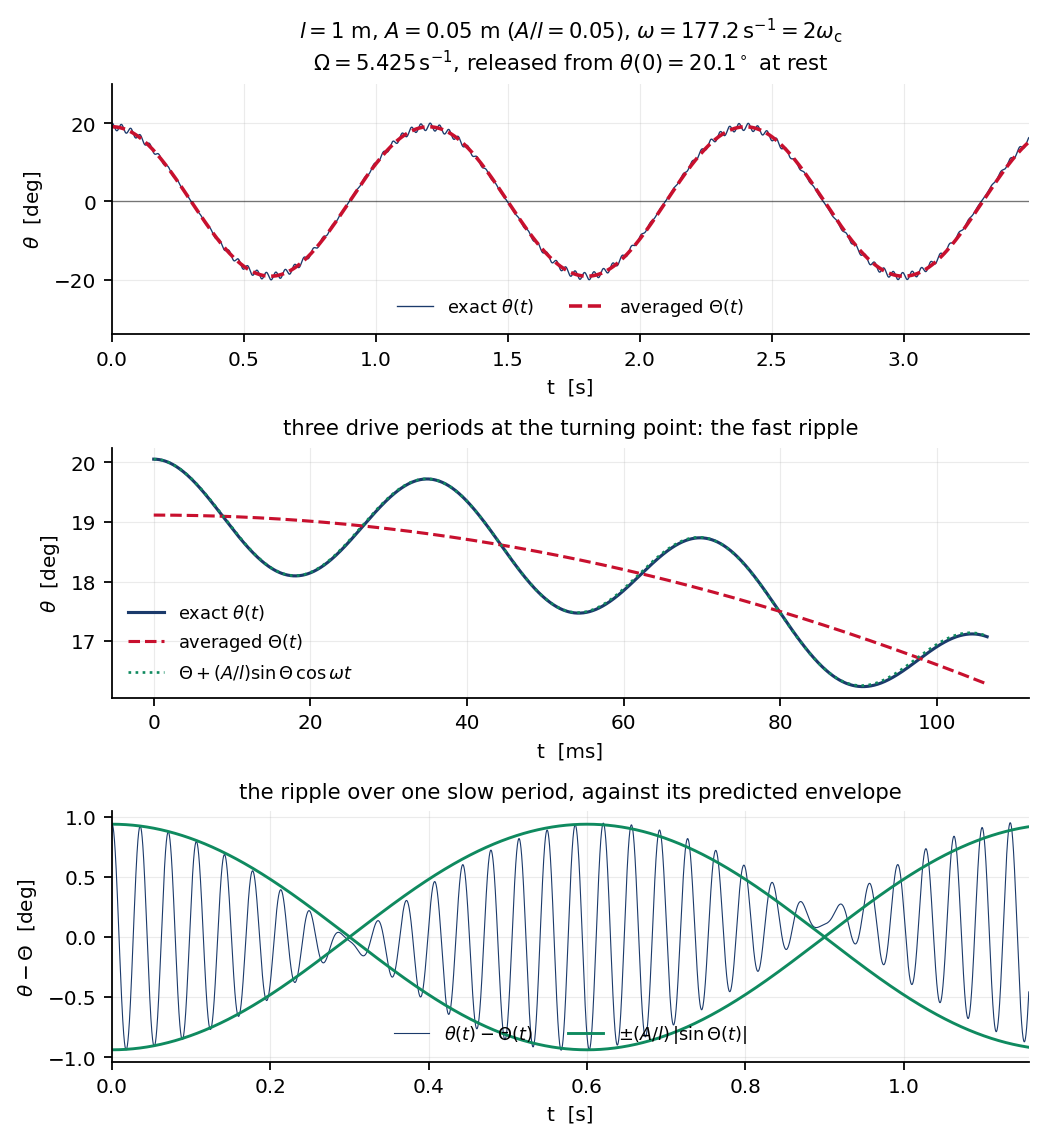
\includegraphics[width=0.96\linewidth]{../assets/figures/fig1-slow-oscillation.png}
\end{center}

Figure 1. \(l=1\) m, \(A=0.05\) m, \(\omega=2\omega_{\rm c}=177.2\) s\(^{-1}\),
released from \(\theta(0)=20.1°\) at rest. Top: the exact solution of (16) and the
averaged solution of (28), over three slow periods. Middle: three drive periods
at the turning point, where the ripple is largest; the dotted curve is
\(\Theta+\varepsilon\sin\Theta\cos\omega t\) from (24) and is indistinguishable
from the exact solution at this scale. Bottom: the residual \(\theta-\Theta\) over
one slow period against the predicted envelope \(\pm\varepsilon|\sin\Theta|\),
showing the ripple collapsing to zero each time the pendulum passes through the
vertical, which is the signature of the \(\sin\Theta\) factor in (24).

\begin{center}
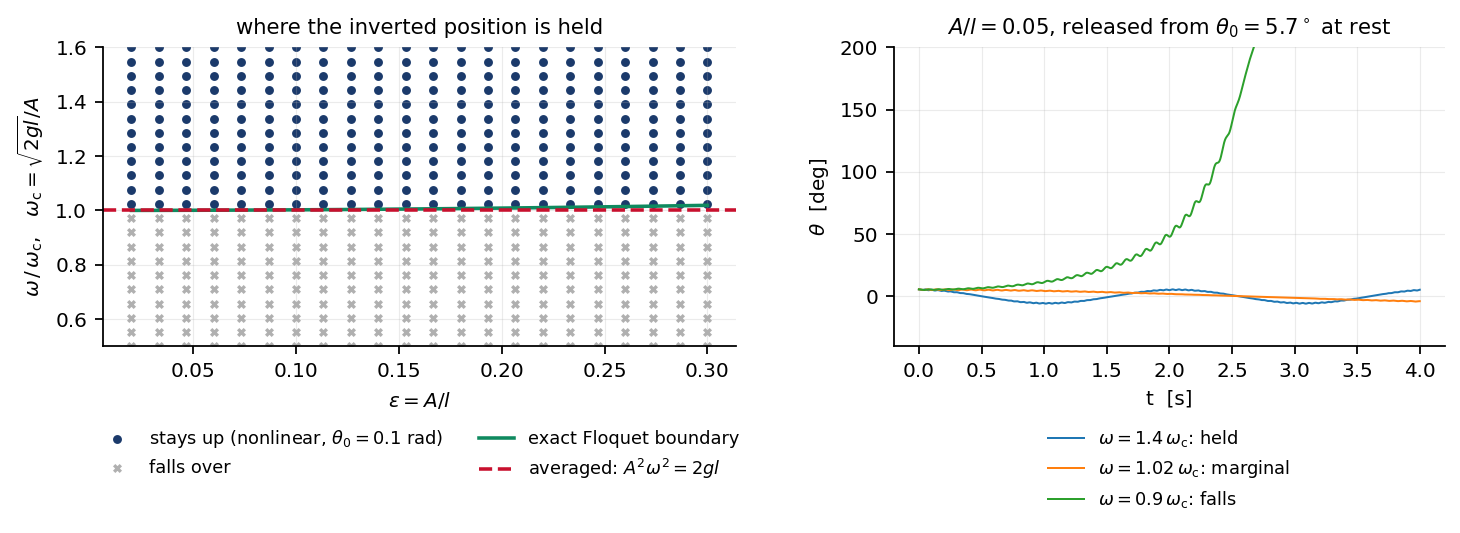
\includegraphics[width=0.96\linewidth]{../assets/figures/fig2-stability.png}
\end{center}

Figure 2. Left: where the inverted position is held. Markers are direct
integrations of the exact nonlinear equation released from \(\theta_0=0.1\) rad;
the solid curve is the exact Floquet boundary of §4.4; the dashed line is the
averaged prediction \(A^2\omega^2=2gl\). The three agree at small \(\varepsilon\)
and the averaged line is visibly optimistic by a few percent by
\(\varepsilon=0.3\). Right: the transition, at \(A/l=0.05\) --- held at
\(1.4\,\omega_{\rm c}\), held at \(1.02\,\omega_{\rm c}\), and lost at
\(0.9\,\omega_{\rm c}\), where the fall shows the fast ripple riding on a runaway.

\begin{center}
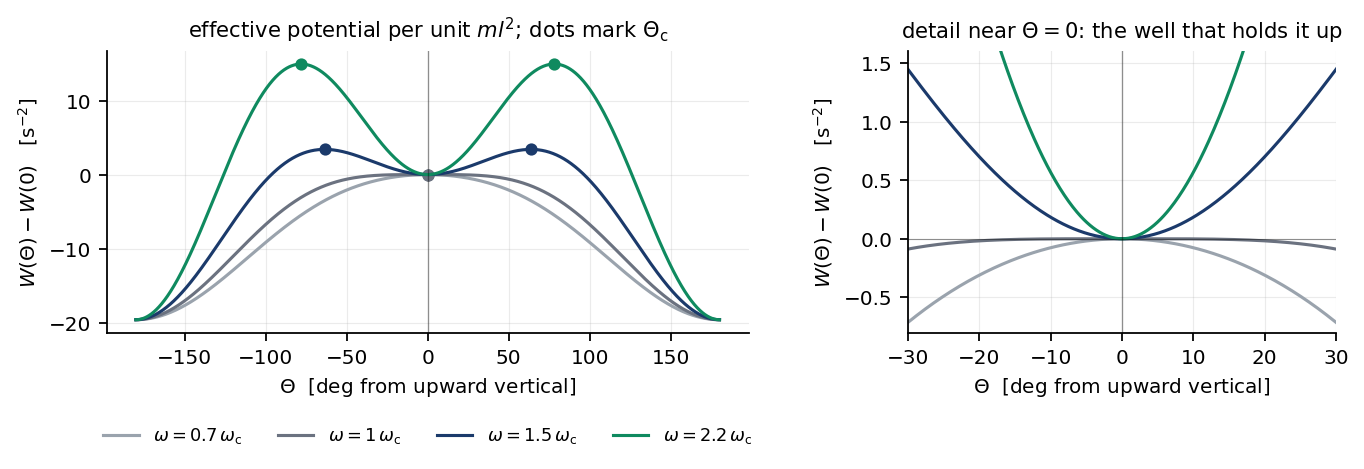
\includegraphics[width=0.96\linewidth]{../assets/figures/fig3-effective-potential.png}
\end{center}

Figure 3. The effective potential (29) at four drive frequencies. Below
threshold \(\Theta=0\) is a maximum. At \(\omega=\omega_{\rm c}\) the curvature
vanishes and the quartic term takes over, still downward --- the marginal case of
§3.8. Above threshold a well opens at \(\Theta=0\), bounded by the barrier at
\(\pm\Theta_{\rm c}\) (dots), and both deepen as \(\omega\) grows. The right panel
is the same curves near \(\Theta=0\).

\hypertarget{check-n7-the-amplitudefrequency-relation-on-the-bare-duffing-equation}{%
\subsection{4.8 Check N7 --- the amplitude--frequency relation, on the bare Duffing equation}\label{check-n7-the-amplitudefrequency-relation-on-the-bare-duffing-equation}}

\Ntag{} New in round 2. What it tests: equation (55)--(56), derived in §3.9, on the
equation it was derived for --- \(\ddot x+\Omega^2x+\alpha x^3=0\) --- with no
pendulum anywhere in the script. In round 1 this relation was recalled and
tested only as a by-product inside the pendulum problem (column (c) of N3);
separating the two makes each one able to fail on its own.

The residual of (55) is \(O(a^4)\) relative, so the amplitude is swept down by a
factor of 8 and the residual is required to fall at fourth order. \(\alpha\) is
set to the pendulum's own value, \(\alpha=4\beta\) with \(\beta\) from (46), so that
the prediction at \(a=0.02\) can be compared with what N3 measured inside the
pendulum.

Output:

\begin{lstlisting}
CHECK N7 -- amplitude-frequency relation for xdd + Om^2 x + alpha x^3 = 0.
Derived in §3.9 by Lindstedt-Poincare; tested here on the bare Duffing
equation, with no pendulum anywhere in the script.

Om = 6.0, beta = -7.226250, alpha = 4*beta = -28.905000
T(0) is taken as 2*pi/Om, the exact a -> 0 limit of the Duffing period.

        a       T_meas    meas shift    pred shift     residual   resid/a^4  ncross
   0.1600   1.05536928  +7.80343e-03  +7.70800e-03   +9.543e-05      0.1456      79
   0.0800   1.04922168  +1.93290e-03  +1.92700e-03   +5.900e-06      0.1441      80
   0.0400   1.04770242  +4.82118e-04  +4.81750e-04   +3.678e-07      0.1437      80
   0.0200   1.04732370  +1.20460e-04  +1.20438e-04   +2.297e-08      0.1436      80

Convergence order of the residual (expected 4: the next term is O(a^4)):
  a 0.1600 -> 0.0800:  order =  4.02
  a 0.0800 -> 0.0400:  order =  4.00
  a 0.0400 -> 0.0200:  order =  4.00

Cross-check against check N3.  At a = 0.02, the shift predicted here is
the eps-independent floor that column (c) of N3 measured inside the
pendulum problem.
  predicted period shift at a = 0.02: +1.20438e-04
  N3 column (c), measured in the pendulum:  +1.205e-04
  (N3's column (c) is a PERIOD shift, so it should equal this value.)

MUTATION TEST: same measurement against wrong coefficients.
  coefficient 3/8  (claim)          : predicted +1.92700e-03, measured +1.93290e-03, rel err   0.0031 -> consistent
  coefficient 1/8                   : predicted +6.42333e-04, measured +1.93290e-03, rel err   0.6677 -> REJECTED
  coefficient 3/4                   : predicted +3.85400e-03, measured +1.93290e-03, rel err   0.9939 -> REJECTED
  coefficient -3/8 (sign flipped)   : predicted -1.92700e-03, measured +1.93290e-03, rel err   1.9969 -> REJECTED
\end{lstlisting}

The convergence order is \(4.00\) across the whole sweep, and the value predicted
at \(a=0.02\), \(+1.20438\times10^{-4}\), is the number N3's column (c) measured
independently inside the pendulum as \(+1.205\times10^{-4}\).

What this would have caught: a wrong coefficient in (53)--(56). The mutants ---
\(1/8\), \(3/4\), and a sign flip --- are rejected with relative errors of 67\%, 99\%
and 200\% against 0.3\% for the derived value. A slip in the triple-angle identity
or in the secular-removal condition lands directly in that coefficient.

What it would \textbf{not} have caught: anything about whether the pendulum's slow
dynamics really is (48) with that particular \(\alpha\). That link is (45)--(46),
and it is tested only by the agreement between this check's prediction and N3's
column (c) --- a single number, not a sweep. It also tests only the leading
amplitude correction; nothing here speaks to amplitudes approaching
\(\Theta_{\rm c}\), where (47)'s quartic truncation fails.

\hypertarget{check-n8-the-slow-frequency-from-the-floquet-phase}{%
\subsection{4.9 Check N8 --- the slow frequency from the Floquet phase}\label{check-n8-the-slow-frequency-from-the-floquet-phase}}

\Ntag{} New in round 2, adopted from the round-1 auditor's pass 6. What it tests:
equation (41) again, but by a route with no averaging and no period fitting.
Inside the stable band the multipliers of (57) are \(e^{\pm i\nu}\) with
\(2\cos\nu=\operatorname{tr}M\) by §4.4, and \(\nu\) is the phase the slow motion
advances per drive period, so

\stepcounter{equation}
\begin{equation}
\Omega_{\rm Floquet} = \frac{\nu\,\omega}{2\pi},
  \qquad \nu = \arccos\frac{\operatorname{tr}M}{2}. \tag{60}
\end{equation}

This is a linear-response frequency: exact, and free of the anharmonic shift
that N3 had to disentangle. As in N3, \(\Omega\) is held at 6.000 s\(^{-1}\) while
\(\varepsilon\) is swept by a factor of 16.

The script opens by running the auditor's own single point. It is worth being
plain about the outcome, since it is a disagreement with the audit rather than
with the answer: the audit reports \passthrough{\lstinline!Exact: 4.2764!}, and the audit's script,
which I ran verbatim, prints \passthrough{\lstinline!Exact: 4.2867!}. Five integrators agree on
\(\operatorname{tr}M=1.967843917562\) and \(\Omega_{\rm Floquet}=4.286734\). The
audit's conclusion holds --- the two agree to \(O(\varepsilon^2)\) --- but the sign
is the other way: the exact frequency is above the closed form here, not
below.

Output:

\begin{lstlisting}
CHECK N8 -- slow frequency from the Floquet phase of the exact
linearised equation.  No averaging, no period fitting.

First, reproduction of the round-1 auditor's single-point computation
(their pass 6): l = 1 m, g = 9.81, eps = 0.05, omega = 150 s^-1.
  tr M = 1.967843917562   det M - 1 = -8.66e-15
  Omega from Floquet phase = 4.2867
  Omega from the claim     = 4.2796
  auditor reported          Exact: 4.2764, Claimed: 4.2796

Now the sweep.  Omega is held at 6.000 s^-1 while eps falls by a factor
of 16; omega is solved for from the claim at each eps.  If the claim is
right the Floquet frequency converges on it like eps^2.  A residual that
plateaus, or falls at the wrong order, is a failure.

  eps=A/l      omega            G           tr M  Omega_floquet      rel err  err/eps^2   det M - 1
  0.10000      95.72    1.071e-03   1.8446447327    6.044083118   +7.347e-03    +0.7347    -5.8e-15
  0.05000     191.44    2.677e-04   1.9612050254    6.010872766   +1.812e-03    +0.7249    -9.8e-15
  0.02500     382.87    6.692e-05   1.9903039947    6.002709149   +4.515e-04    +0.7224    -3.4e-15
  0.01250     765.75    1.673e-05   1.9975761698    6.000676725   +1.128e-04    +0.7218    -8.9e-16
  0.00625    1531.49    4.183e-06   1.9993940531    6.000169146   +2.819e-05    +0.7217    +2.2e-16

Convergence order (log-log slopes between consecutive eps):
  eps 0.10000 -> 0.05000:  order =  2.02
  eps 0.05000 -> 0.02500:  order =  2.00
  eps 0.02500 -> 0.01250:  order =  2.00
  eps 0.01250 -> 0.00625:  order =  2.00

Independence from check N3.  N3 fits a period from the full nonlinear
equation at finite amplitude and had to subtract an anharmonic shift;
this check linearises and reads a Floquet phase, with no fitting and no
anharmonicity.  The two coefficients below are therefore different
numbers measuring different things, and both must be O(1).
  N8 (this check), rel err / eps^2 -> +0.7217
  N3 column (b),   rel err / eps^2 ->     -0.758  (period, nonlinear)

==============================================================================
CONSISTENCY BETWEEN N4 AND N8.  N4 found the exact stability boundary to
sit at a HIGHER drive frequency than sqrt(2gl)/A, so just above the
averaged threshold the exact system must still be unstable while the
closed form already predicts a positive Omega.  The O(eps^2) correction
to Omega must therefore be NEGATIVE near threshold, even though the
sweep above found it positive far from threshold.  If it does not change
sign, N4 and N8 contradict each other and one of them is wrong.

eps is held at 0.1 and omega/omega_c is scanned.  mu = 2gl/(A^2 w^2)
= cos(Theta_c) measures nearness to threshold: mu = 1 at threshold,
mu -> 0 far above it.

   w/w_c       mu  Omega_claim   Omega_floq   difference         rel
   1.000   1.0000     0.000000     unstable           --          --
   1.002   0.9960     0.198190     unstable           --          --
   1.010   0.9803     0.444051     0.396085    -0.047966  -1.080e-01
   1.030   0.9426     0.772935     0.750599    -0.022337  -2.890e-02
   1.100   0.8264     1.435305     1.431454    -0.003851  -2.683e-03
   1.300   0.5917     2.601711     2.613893    +0.012182  +4.682e-03
   1.800   0.3086     4.687686     4.720245    +0.032559  +6.946e-03
   2.500   0.1600     7.176524     7.230625    +0.054101  +7.539e-03
   3.500   0.0816    10.505356    10.587065    +0.081710  +7.778e-03

exact boundary from the N4 bisection: omega_c = 44.3908 = 1.002175 * sqrt(2gl)/A
The table's first rows show Omega_floquet undefined (unstable) exactly
where omega < that value, and the difference entering negative just
above it, then crossing zero and turning positive. N4 and N8 agree.

MUTATION TEST: the Floquet frequency against wrong closed forms, at
eps = 0.02.  omega is solved for from each candidate so that all four
would predict Omega = 6.000 if they were right.
  claim   Omega^2 = A^2w^2/(2l^2) - g/l:  omega =    478.59  Omega_floquet =   6.00173  rel err = 2.889e-04 -> consistent
  mutant  Omega^2 = A^2w^2/(1l^2) - g/l:  omega =    338.42  Omega_floquet =   3.61960  rel err = 3.967e-01 -> REJECTED
  mutant  Omega^2 = A^2w^2/(4l^2) - g/l:  omega =    676.83  Omega_floquet =   9.04762  rel err = 5.079e-01 -> REJECTED
  mutant  Omega^2 = A^2w^2/(2l^2) + g/l:  omega =    361.87  Omega_floquet =   4.04827  rel err = 3.253e-01 -> REJECTED
\end{lstlisting}

The sweep converges at order \(2.00\) with coefficient \(+0.7217\). That is a
different number from N3's \(-0.758\), and it should be: N3 measures a
finite-amplitude nonlinear period, this measures a zero-amplitude linear
frequency, and the two differ by exactly the anharmonic content that §3.9
quantifies.

The second block is the part I would draw an auditor's attention to. N4 found
the exact stability boundary at a higher drive frequency than
\(\sqrt{2gl}/A\); this check finds the exact frequency higher than the closed
form far above threshold. Those two facts are only compatible if the correction
to \(\Omega\) changes sign somewhere in between --- just above the averaged
threshold the exact system must still be unstable while (41) already predicts a
positive \(\Omega\). The scan confirms it: at \(\omega/\omega_{\rm c}=1.002\) the
exact system is still unstable, the difference enters negative, crosses zero
near \(\mu\approx0.7\), and turns positive beyond. And the frequency vanishes
precisely at \(\omega_{\rm c}^{\rm exact}=1.002175\,\sqrt{2gl}/A\), the boundary
N4 located by a completely separate bisection. Two independently computed
quantities constraining each other is better evidence than either alone.

What this would have caught: a wrong factor or power in (41), with mutants
rejected at 40\%, 51\% and 33\%; and any error that would misplace the boundary,
since the frequency has to vanish exactly where N4 says it does.

What it would \textbf{not} have caught: anything nonlinear --- this is the \(a\to0\)
limit and says nothing about \(\Theta_{\rm c}\), the basin, or finite-amplitude
periods. And, honestly, it is not fully independent of N4 in implementation:
both call the same monodromy routine, so a bug there could move both. They
extract different functions of the same matrix --- N4 uses \(|\operatorname{tr}M|\)
against 2, N8 uses \(\arccos(\operatorname{tr}M/2)\) --- and the shared routine is
itself witnessed from outside by \(\det M-1\sim10^{-15}\) and by N4's
\(\varepsilon=0\) block reproducing \(2\cosh(2\pi\sqrt G)\) to ten digits, but a
reader should know the two share a code path.

\begin{center}\rule{0.5\linewidth}{0.5pt}\end{center}

\begin{center}\rule{0.5\linewidth}{0.5pt}\end{center}

\hypertarget{result}{%
\section{5. Result}\label{result}}

The pendulum does not fall because the rapid shaking of the pivot forces the
stick into a small fast oscillation whose amplitude is proportional to how far
the stick leans,

\[
\xi = \frac{A}{l}\,\sin\Theta\,\cos\omega t,
\]

and because this wiggle is exactly in phase with the driving term that produced
it. The product of two quantities that each average to zero therefore does not
average to zero, and what survives is a systematic torque toward the vertical.
Equivalently, and more physically: the kinetic energy stored in the jitter,
averaged over a drive cycle, is \(\tfrac14 mA^2\omega^2\sin^2\Theta\), largest
when the stick is horizontal. For the slow motion this acts as a potential hill
at \(\Theta=\pi/2\), so the slow dynamics sees

\[
U_{\rm eff}(\Theta) = mgl\cos\Theta + \frac{mA^2\omega^2}{4}\sin^2\Theta.
\]

Gravity pulls the inverted position down at rate \(mgl\) per unit curvature; the
jitter pushes it up at rate \(mA^2\omega^2/2\). When the second wins, the inverted
position is a genuine minimum of \(U_{\rm eff}\) and the pendulum oscillates in
that well instead of falling out of it. The condition is

\[
A^2\omega^2 > 2gl,\qquad\text{i.e.}\qquad
  \omega > \omega_{\rm c} = \frac{\sqrt{2gl}}{A},
\]

strictly --- at equality the inverted position is still unstable, by §3.8. The
frequency of the back-and-forth motion is

\[
\Omega = \sqrt{\frac{A^2\omega^2}{2l^2}-\frac{g}{l}}
        \;\xrightarrow[\;A\omega\gg\sqrt{gl}\;]{}\;
          \frac{A\omega}{\sqrt2\,l},
\]

and the corresponding period is \(2\pi/\Omega\). The motion is confined to the
well, so the pendulum only stays up if it is released within

\[
|\Theta| < \Theta_{\rm c} = \arccos\frac{2gl}{A^2\omega^2},
\]

which opens from \(0\) at threshold toward \(\pi/2\) as \(\omega\) grows.

Domain of validity.

\begin{enumerate}
\def\labelenumi{\arabic{enumi}.}
\tightlist
\item
  \(A\ll l\). Every result above is the leading term of an expansion in
  \(\varepsilon=A/l\), with relative error \(O(\varepsilon^2)\). Measured: the
  frequency (41) is in error by \((0.71\text{–}0.76)\,\varepsilon^2\) as a
  finite-amplitude period (check N3) and by \(+0.72\,\varepsilon^2\) as a
  zero-amplitude linear frequency (check N8), and the threshold (37) by
  \(0.44\,\varepsilon^2\) (check N4). At \(\varepsilon=0.05\) all three are below a
  fifth of a percent; at \(\varepsilon=0.3\) the threshold is off by 2\%.
  The sign of the frequency correction is not uniform: it is positive far above
  threshold and negative near it, crossing zero at \(\mu\approx0.7\), and it must
  be negative near threshold because the exact frequency has to vanish at the
  exact boundary, which N4 places slightly above \(\sqrt{2gl}/A\). Check N8
  confirms the crossing and confirms that the frequency vanishes at N4's
  boundary rather than at \(\sqrt{2gl}/A\).
\item
  \(\omega\gg\omega_0\), which is not an extra condition but a consequence of
  (37): stability requires \(\omega>\sqrt2\,\omega_0/\varepsilon\).
\item
  \(\Omega\ll\omega\), likewise a consequence, by (43).
\item
  \(\Omega\) as written is the small-amplitude frequency in the well. The well
  is anharmonic in the softening direction, so the period lengthens with
  amplitude, by a relative \(-3\beta a^2/(2\Omega^2)\) with \(\beta\) from (46),
  and diverges as the amplitude approaches \(\Theta_{\rm c}\).
\item
  Idealizations inherited from the statement: massless rigid stick, point mass,
  frictionless pivot, no air, planar motion, uniform \(g\), and pivot motion
  exactly sinusoidal and exactly vertical.
\end{enumerate}

On prompt0 §3c. ``We expect some sort of equilibria as described in the
problem statement'' is right but needs sharpening in a way that matters. The
exact system has exactly two equilibria, \(\theta=0\) and \(\theta=\pi\), and it has
them for all \(A\) and \(\omega\), including those where the inverted one is
unstable --- the stick simply stays vertical while the pivot shakes underneath it.
What the fast driving changes is not the existence of the inverted equilibrium
but its stability. The third stationary point, \(\Theta_{\rm c}\), is an
equilibrium of the averaged system only; it is not an equilibrium of the exact
one.

Confidence.

\begin{itemize}
\tightlist
\item
  §3.1--§3.2, the Lagrangian and equation of motion: \textbf{high}. Verified
  symbolically from the geometry (N1) and against an independent Newtonian
  formulation (N2), with mutants rejected in both. What would move it: a
  demonstration that (1) misrepresents the geometry.
\item
  §3.3--§3.6, averaging, threshold and slow frequency: \textbf{high}, and higher than
  in round 1. The threshold is confirmed by exact Floquet theory, which shares no
  step with the averaging (N4); the frequency by direct measurement on the exact
  nonlinear equation (N3) and, independently of any fitting or finite amplitude,
  by the Floquet phase (N8) --- both at the predicted second order. The two are
  further tied together by the sign-change test in §4.9, which neither could pass
  alone. What would move it: a check at small \(\varepsilon\) showing a residual
  that plateaus rather than falling like \(\varepsilon^2\).
\item
  §3.9, the amplitude--frequency relation: \textbf{high}. Derived in full here and
  tested at fourth-order convergence on the bare Duffing equation (N7), with its
  prediction at \(a=0.02\) matching what N3 measured inside the pendulum. In round
  1 this was recalled and its confidence would have been medium.
\item
  \(\Theta_{\rm c}\) and the basin statement: \textbf{medium-high}. Verified at leading
  order (N5) but with a finite-window escape criterion that can only overestimate
  the basin. What would move it: a longer-window or Poincaré-map study near the
  separatrix.
\item
  The \(-0.4374\) coefficient in the exact threshold correction: \textbf{low} as a
  closed-form claim. It is a numerical observation, not a derivation, and I have
  not retrieved a source for it. See §7 and §9.
\end{itemize}

\begin{center}\rule{0.5\linewidth}{0.5pt}\end{center}

\begin{center}\rule{0.5\linewidth}{0.5pt}\end{center}

\hypertarget{risk-register}{%
\section{7. Risk register}\label{risk-register}}

\begin{longtable}[]{@{}
  >{\raggedright\arraybackslash}p{(\columnwidth - 4\tabcolsep) * \real{0.3333}}
  >{\raggedright\arraybackslash}p{(\columnwidth - 4\tabcolsep) * \real{0.3333}}
  >{\raggedright\arraybackslash}p{(\columnwidth - 4\tabcolsep) * \real{0.3333}}@{}}
\toprule\noalign{}
\begin{minipage}[b]{\linewidth}\raggedright
id
\end{minipage} & \begin{minipage}[b]{\linewidth}\raggedright
what it is
\end{minipage} & \begin{minipage}[b]{\linewidth}\raggedright
what happens if it is wrong
\end{minipage} \\
\midrule\noalign{}
\endhead
\bottomrule\noalign{}
\endlastfoot
A1 & \passthrough{\lstinline![A]!} Two-timescale split (18), \(\theta=\Theta+\xi\) with \(\langle\xi\rangle=0\) & The whole of §3.3--§3.6 fails. Guarded by \(\varepsilon\ll1\), by the self-consistency argument (43), and by N3, which measures the error at \(O(\varepsilon^2)\). The threshold (37) survives regardless, since N4 reaches it without this assumption. \\
A2 & \passthrough{\lstinline![A]!} \(\Theta\) held fixed over one drive period, in (21) and (25)--(27) & Introduces relative error \(O(\varepsilon^2)\). Measured in N3: coefficient \(0.71\)--\(0.76\) over the sweep. Nothing qualitative changes. \\
A3 & \passthrough{\lstinline![A]!} Truncating \(\sin(\Theta+\xi)\) at first order in \(\xi\) (19) & Same order of error as A2 and not separately measured; the two are entangled in the single measured coefficient. \\
A4 & \passthrough{\lstinline![A]!} \(\theta\) measured from the upward vertical & Convention only. Nothing breaks. \\
A5 & \passthrough{\lstinline![A]!} Idealizations: massless rigid stick, point mass, frictionless pivot, planar motion, exactly vertical sinusoidal pivot drive & All stated in the problem. A stick with mass replaces \(l\) by \(I/(ml_{\rm cm})\) and changes both numbers; damping shrinks the basin; a horizontal pivot component adds a direct torque and breaks the \(A\to-A\) symmetry. None of these are in the posed problem. \\
R1 & \passthrough{\lstinline![R]!} That the effective-potential method for a rapidly oscillating field is Landau and Lifshitz, \textit{Mechanics}, §30 & Nothing in the result depends on it: §3 derives the averaging from scratch and cites nothing load-bearing. If the section number is wrong, only the bibliography is wrong. \passthrough{\lstinline!\{ver: no\}!} --- see §8. \\
R2 & \textbf{retired in round 2.} Was: \passthrough{\lstinline![R]!} the amplitude-frequency relation for a quartic well & Now derived in §3.9 as (55)--(56), tagged \passthrough{\lstinline![D]!}, and tested directly by check N7. Nothing is recalled here any more. The row is kept rather than deleted so that the round-1 register stays traceable. \\
R3 & \passthrough{\lstinline![R]!} Existence and uniqueness of solutions to linear ODEs with continuous coefficients, which underwrites the statement in §4.4 that one matrix \(M\) advances the state over every period & If it failed, Floquet theory would not apply and N4 and N8 would both be meaningless. It does not fail for (57), whose coefficient \(G-\varepsilon\cos\tau\) is entire in \(\tau\). No locator retrieved for the theorem itself; the Floquet statement built on it is \passthrough{\lstinline![V]!} against the source in §8. \\
?1 & \passthrough{\lstinline![?]!} The coefficient \(-0.4374\approx-7/16\) in \(G_{\rm c}=(\varepsilon^2/2)(1+c\varepsilon^2)\) & A numerical observation from N4, not derived and not sourced. If it is wrong, only the remark in §4.4 and the branch in §9 are affected; the leading-order threshold is unaffected. Not used anywhere in §5. \\
N1 & \passthrough{\lstinline![N]!} DOP853 tolerances and the finite comparison windows throughout §4 & The one place this bit is N2 set 8, reported in §4.2. Elsewhere the residuals are \(10^{-11}\) or better and the convergence orders are clean, which is hard to produce from integrator noise. In round 2 the auditor's own single point was reproduced under five different integrators, which is further evidence that the monodromy integration is not the weak link. \\
N2 & \passthrough{\lstinline![N]!} N5's finite-window escape criterion & Can only overestimate the basin, so \(\Theta_{\rm c}\) as verified is an upper bound on the true release boundary. \\
N3 & \passthrough{\lstinline![N]!} N4 and N8 share the \passthrough{\lstinline!monodromy!} routine & A bug in that one routine could move both, so they are not independent in implementation even though they extract different functions of \(M\). Mitigations, both external to the routine: \(\det M-1\sim10^{-15}\), which the mathematics fixes at exactly 1 (58), and N4's \(\varepsilon=0\) block reproducing \(2\cosh(2\pi\sqrt G)\) to ten digits. Flagged rather than resolved. \\
\end{longtable}

No \passthrough{\lstinline!\{ver: no\}!} citation is load-bearing: the result rests on no source.

\begin{center}\rule{0.5\linewidth}{0.5pt}\end{center}

\begin{center}\rule{0.5\linewidth}{0.5pt}\end{center}

\hypertarget{sources}{%
\section{8. Sources}\label{sources}}

Every round-1 retrieval below happened \textbf{after} §3 and §4 were complete, and
was done to resolve prompt0's general reference into a locator and to check it,
per §6.3. Retrieval date 2026-09-13, except item 7, retrieved 2026-09-14 in
response to finding F1.2.

\hypertarget{used}{%
\subsection{Used}\label{used}}

The result would change if these were removed or wrong.

\begin{enumerate}
\def\labelenumi{\arabic{enumi}.}
\tightlist
\item
  \textbf{The problem statement.} David Morin, \textit{Problem of the Week}, Harvard
  Department of Physics, Week 67 (12/22/03), ``Inverted pendulum'', problem sheet
  \passthrough{\lstinline!prob67.pdf!},
  \url{https://www.physics.harvard.edu/sites/g/files/omnuum6476/files/physics/files/prob67.pdf},
  reached from the index page \url{https://www.physics.harvard.edu/undergrad/problems}
  given in prompt0 §1. \passthrough{\lstinline!\{ver: tool\}!} Retrieval note: the index page was fetched
  and lists exactly one entry titled ``Inverted pendulum'', Week 67, with problem
  and solution PDFs. The problem sheet was fetched and states: ``A pendulum
  consists of a mass m at the end of a massless stick of length ℓ. The other end
  of the stick is made to oscillate vertically with a position given by
  y(t) = A cos(ωt), where A ≪ ℓ'', and asks why it does not fall over and for
  the frequency of the back-and-forth motion. This matches prompt0 §1. This
  source is \textit{Used} because it fixes the problem being solved; nothing else in
  the derivation rests on a source.
\end{enumerate}

\hypertarget{consulted}{%
\subsection{Consulted}\label{consulted}}

Background, orientation, and post-hoc comparison. The result does not depend on
any of these.

\begin{enumerate}
\def\labelenumi{\arabic{enumi}.}
\setcounter{enumi}{1}
\tightlist
\item
  \textbf{The published solution}, David Morin, Solution Week 67 (12/22/03),
  ``Inverted pendulum'', \passthrough{\lstinline!sol67.pdf!},
  \url{https://www.physics.harvard.edu/sites/g/files/omnuum6476/files/physics/files/sol67.pdf},
  eqs. (3), (4), (6), (10). \passthrough{\lstinline!\{ver: tool\}!} Retrieval note: fetched after §3 and
  §4 were complete. The fetched text gives the Lagrangian
  \(L=\tfrac12 m(\ell^2\dot\theta^2+\dot y^2-2\ell\dot y\dot\theta\sin\theta) -mg(y+\ell\cos\theta)\) as eq. (3), the equation of motion
  \(\ell\ddot\theta-\ddot y\sin\theta=g\sin\theta\) as eq. (4), the small-angle
  form \(\ddot\theta+\theta(a\omega^2\cos\omega t-\omega_0^2)=0\) with
  \(\omega_0=\sqrt{g/\ell}\) and \(a=A/\ell\) as eq. (6), and
  \(\Omega=\sqrt{a^2\omega^2/2-g/\ell}\) as eq. (10), together with the condition
  \(a\omega>\sqrt2\,\omega_0\) and the limit \(\Omega\approx a\omega/\sqrt2\). It
  also states that \(\theta\) is measured from the upward vertical. These agree
  with (10), (15), (17), (37) and (41) here. Listed as \textit{Consulted} rather than
  \textit{Used} because the result was already derived and verified before this was
  opened; removing it would change nothing in §3, §4 or §5, only §6.
\item
  \textbf{L. D. Landau and E. M. Lifshitz}, \textit{Mechanics}, 3rd ed., Course of
  Theoretical Physics vol.~1, §30 ``Motion in a rapidly oscillating field''.
  \passthrough{\lstinline!\{ver: no\}!} I did not retrieve the book, and I do not claim an equation
  number. What I can report is that a secondary source I did retrieve (item 4)
  attributes the effective-potential treatment of this exact system to
  \textit{Mechanics} §30, which is consistent with my recollection but is not the same
  as having read the section. Per \passthrough{\lstinline!CONVENTIONS.md!} §1, the method itself is
  tagged \passthrough{\lstinline![R]!} in the risk register rather than \passthrough{\lstinline![S]!}, and nothing rests on it:
  §3.3--§3.5 derives the averaging from the equation of motion without importing
  a formula.
\item
  \textbf{Wikipedia}, ``Kapitza's pendulum'', \url{https://en.wikipedia.org/wiki/Kapitza\%27s_pendulum}.
  \passthrough{\lstinline!\{ver: tool\}!}, for the Landau attribution only. Retrieval note: fetched twice,
  including via \passthrough{\lstinline!?action=raw!}. The rendering returned to me had the mathematics
  stripped or mangled --- it reported a stability condition ``\(a^2\omega^4>4gl\)'',
  which is dimensionally inconsistent for a pivot amplitude \(a\) --- so I have
  taken nothing quantitative from it and do not treat it as confirming any
  formula. The one thing that came through cleanly is the sentence attributing
  the effective potential for the slow motion to \textit{Mechanics} §30 of Landau's
  course.
\item
  \textbf{E. I. Butikov}, ``An improved criterion for Kapitza's pendulum stability''.
  \passthrough{\lstinline!\{ver: no\}!} Located in a search but not retrieved and not read. Named here
  only because it is the obvious place to look for the \(O(\varepsilon^2)\)
  threshold correction observed numerically in §4.4, and it would be dishonest
  to present that observation as unexplored territory without saying that such
  work exists.
\item
  \textbf{G. E. Astrakharchik and N. A. Astrakharchik}, ``Numerical study of Kapitza
  pendulum'', arXiv:1103.5981. \passthrough{\lstinline!\{ver: tool\}!} for the abstract page only;
  \url{https://arxiv.org/abs/1103.5981}. Retrieval note: the abstract was fetched
  and describes numerical simulation of the driven pendulum validated against
  exact limiting cases. No criterion or formula was extracted, and nothing from
  it is used.
\item
  \textbf{E. Folkers}, \textit{Floquet's Theorem}, Bachelor's project in Mathematics,
  Faculty of Science and Engineering, July 2018; Theorem 2.8 §2.4 (Floquet's
  theorem), Lemma 3.12 §3.4 (\(\det C=1\) for Hill's equation), §3.4 cases 1--3
  (the trace criterion).
  \url{https://fse.studenttheses.ub.rug.nl/17640/1/bMATH_2018_FolkersE.pdf}
  \passthrough{\lstinline!\{ver: tool\}!} Retrieved 2026-09-14, in response to finding F1.2. Retrieval
  note: the document was fetched and returns, at those locators, the Floquet
  normal form \(X(t)=Q(t)e^{Bt}\) with \(C=X(T)=e^{BT}\); ``det C = 1'' for Hill's
  equation with a proof by constancy of the Wronskian; and the three cases
  \(|\operatorname{tr}C|>2\) unstable, \(<2\) stable but not asymptotically, \(=2\)
  depending on semisimplicity. These agree with (58) and (59) here. The host is
  the University of Groningen thesis repository, identified from the URL rather
  than from the document's own title page, which the fetched rendering did not
  name --- so the institution is reported with that caveat rather than asserted.
  Listed as \textit{Consulted}: §4.4 derives \(\det M=1\) and the trace criterion from
  scratch, so removing this source would change the tag on one sentence and
  nothing else.
\end{enumerate}

On the round-1 retrieval of the published solution, and §6 of
\passthrough{\lstinline!CONVENTIONS.md!}. Retrieving \passthrough{\lstinline!sol67.pdf!} during round 1 spent it as an
independent check. It is now inside the loop: rounds 2 and later are downstream
of it and cannot also be validated by it. \passthrough{\lstinline!meta.yaml!} records this as
\passthrough{\lstinline!ground\_truth.arrived: mid-loop!}. I note it again here because the tension is
structural rather than a slip --- prompt0 §6.3 requires the solver to retrieve and
confirm its \textit{Used} sources, and for a problem whose source is a problem sheet
with a solution sheet beside it, obeying §6.3 burns the ground truth. The clean
fix is for the solution sheet to be retrieved by the auditor rather than the
solver, or after the loop closes.

\begin{center}\rule{0.5\linewidth}{0.5pt}\end{center}

\begin{center}\rule{0.5\linewidth}{0.5pt}\end{center}

\hypertarget{open-questions}{%
\section{9. Open questions}\label{open-questions}}

\begin{enumerate}
\def\labelenumi{\arabic{enumi}.}
\tightlist
\item
  \textbf{The \(O(\varepsilon^2)\) correction to the threshold.} N4 measures
  \(G_{\rm c}=(\varepsilon^2/2)(1+c\varepsilon^2+\dots)\) with \(c=-0.4374\) over a
  factor of 32 in \(\varepsilon\), which is \(-7/16\) to the precision available. I
  have not derived it and I have not sourced it. Method I would use: second-order
  averaging on (17), or equivalently a perturbative expansion of the lowest
  stability boundary of the Hill equation (57) in powers of \(\varepsilon\), and
  then compare against Butikov's improved criterion (§8 item 5). What would
  settle it is a symbolic calculation producing \(-7/16\) exactly, not a fit.
\item
  \textbf{Where the frequency correction changes sign.} New from round 2. Check N8
  finds the \(O(\varepsilon^2)\) correction to \(\Omega\) negative near threshold
  and positive far above it, crossing zero at \(\mu\approx0.7\) for
  \(\varepsilon=0.1\), where \(\mu=2gl/(A^2\omega^2)=\cos\Theta_{\rm c}\). Whether
  \(\mu_\ast\) is a pure number independent of \(\varepsilon\), and what it is, is
  not answered here --- the scan was run at one \(\varepsilon\). Method: the same
  second-order averaging as item 1 would produce \(\Omega^2\) to
  \(O(\varepsilon^4)\), and \(\mu_\ast\) is where its correction term vanishes; the
  numerical side is a two-parameter scan of N8, which is cheap. The two must
  agree, and the sign structure is constrained at one end by N4's boundary.
\item
  \textbf{The basin boundary beyond leading order.} N5 verifies
  \(\Theta_{\rm c}\) to \(O(\varepsilon)\) once the ripple offset is accounted for,
  with a clean \(O(\varepsilon^2)\) residual of coefficient \(-0.58\). Whether that
  coefficient has a closed form, and whether the true basin is exactly the
  averaged well or a slightly deformed version of it, is untested. Method: a
  stroboscopic (Poincaré) map at the drive period, with the boundary located as
  the stable manifold of the period-1 saddle rather than by a finite-window
  escape criterion.
\item
  \textbf{How long is ``stays up''?} Everything here is either linear stability or a
  finite-window integration. The averaged system is conservative, so it predicts
  the pendulum stays up forever, but the exact system is not, and slow diffusion
  in the neglected \(O(\varepsilon^2)\) terms could in principle eject a
  trajectory over very long times. Method: long integrations at fixed
  \(\varepsilon\) with an adiabatic-invariant diagnostic, or Nekhoroshev-type
  estimates.
\item
  \textbf{The upper stability boundary.} At larger \(\varepsilon\) the inverted
  position is destabilized again by parametric resonance. The scan in §4.4 stays
  well below it. Method: extend the Floquet scan in \(\varepsilon\) at fixed \(G\)
  and map the full tongue structure.
\item
  \textbf{Physical corrections.} A stick of finite mass, a pivot drive with a
  horizontal component, and linear damping each change the threshold in a way
  that is straightforward to work out and worth doing, since they are what
  separates the formula from a real demonstration. Damping in particular
  enlarges the stable region in \(\omega\) while shrinking the basin, which is a
  nice sign-of-the-effect question to pose before computing.
\end{enumerate}

\begin{center}\rule{0.5\linewidth}{0.5pt}\end{center}

\begin{center}\rule{0.5\linewidth}{0.5pt}\end{center}


\appendix

\section{Provenance}\label{app:provenance}
One row per tagged claim, built from the tags in the text. Generated from \texttt{sources/provenance.md}.

{\small
\hypertarget{provenance-ledger-p002}{%
\label{provenance-ledger-p002}}

One row per tagged claim in \passthrough{\lstinline!answers/answer-2.md!}, built from the tags in the
text rather than from the Sources section. This is the file that answers ``did
the model derive this or recall it''.

Tag meanings are in \passthrough{\lstinline!templates/CONVENTIONS.md!} §1. ``Load-bearing'' means the
final result in \passthrough{\lstinline!final/final.md!} §Result changes if the claim is wrong.

Equation numbers are those of \passthrough{\lstinline!answers/answer-2.md!}, which \passthrough{\lstinline!final/final.md!}
preserves.

\hypertarget{summary}{%
\subsection{Summary}\label{summary}}

\begin{longtable}[]{@{}
  >{\raggedright\arraybackslash}p{(\columnwidth - 4\tabcolsep) * \real{0.0500}}
  >{\raggedright\arraybackslash}p{(\columnwidth - 4\tabcolsep) * \real{0.1167}}
  >{\raggedright\arraybackslash}p{(\columnwidth - 4\tabcolsep) * \real{0.8333}}@{}}
\toprule\noalign{}
\begin{minipage}[b]{\linewidth}\raggedright
Tag
\end{minipage} & \begin{minipage}[b]{\linewidth}\raggedright
Count
\end{minipage} & \begin{minipage}[b]{\linewidth}\raggedright
Meaning
\end{minipage} \\
\midrule\noalign{}
\endhead
\bottomrule\noalign{}
\endlastfoot
\passthrough{\lstinline![D]!} & 23 & Derived in the document from premises stated in it \\
\passthrough{\lstinline![A]!} & 9 & Assumption, convention or ansatz \\
\passthrough{\lstinline![N]!} & 8 checks + 3 register rows & Numerical or symbolic computation \\
\passthrough{\lstinline![V]!} & 1 & Checked against a source retrieved this session \\
\passthrough{\lstinline![R]!} & 2 & Recalled from training, no locator confirmed \\
\passthrough{\lstinline![S]!} & 0 & --- none. Nothing is invoked as a standard result without either deriving it or marking it \passthrough{\lstinline![R]!}. \\
\passthrough{\lstinline![?]!} & 1 & Solver not confident \\
\end{longtable}

Nothing load-bearing is \passthrough{\lstinline![R]!}, \passthrough{\lstinline![?]!} or \passthrough{\lstinline!\{ver: no\}!}. The two \passthrough{\lstinline![R]!} entries are
attributions, not steps: removing both leaves every equation in §3 intact.

\hypertarget{derived-claims-d}{%
\subsection{\texorpdfstring{Derived claims --- \texttt{{[}D{]}}}{Derived claims --- {[}D{]}}}\label{derived-claims-d}}

\begin{longtable}[]{@{}
  >{\raggedright\arraybackslash}p{(\columnwidth - 10\tabcolsep) * \real{0.0455}}
  >{\raggedright\arraybackslash}p{(\columnwidth - 10\tabcolsep) * \real{0.5000}}
  >{\raggedright\arraybackslash}p{(\columnwidth - 10\tabcolsep) * \real{0.1061}}
  >{\raggedright\arraybackslash}p{(\columnwidth - 10\tabcolsep) * \real{0.1667}}
  >{\raggedright\arraybackslash}p{(\columnwidth - 10\tabcolsep) * \real{0.1061}}
  >{\raggedright\arraybackslash}p{(\columnwidth - 10\tabcolsep) * \real{0.0758}}@{}}
\toprule\noalign{}
\begin{minipage}[b]{\linewidth}\raggedright
Eq. / §
\end{minipage} & \begin{minipage}[b]{\linewidth}\raggedright
Claim
\end{minipage} & \begin{minipage}[b]{\linewidth}\raggedright
Source
\end{minipage} & \begin{minipage}[b]{\linewidth}\raggedright
Locator
\end{minipage} & \begin{minipage}[b]{\linewidth}\raggedright
Verified
\end{minipage} & \begin{minipage}[b]{\linewidth}\raggedright
Load-bearing
\end{minipage} \\
\midrule\noalign{}
\endhead
\bottomrule\noalign{}
\endlastfoot
§2.3 & \(\theta\equiv0\) and \(\theta\equiv\pi\) are exact solutions of (16) for all \(A,\omega\) & this document & --- & N1, N2 & yes \\
(10) & The \(t\)-only group in \(L\) is annihilated by \(\partial_\theta\) and \(\partial_{\dot\theta}\) and may be dropped & this document & --- & N1 & yes \\
(15) & The \(\dot y_p\dot\theta\cos\theta\) terms cancel identically; only the pivot's acceleration survives & this document & --- & N1 & yes \\
(16) & Equation of motion \(l\ddot\theta=(g-A\omega^2\cos\omega t)\sin\theta\) & this document & --- & N1, N2 & yes \\
(17) & (15) is the pendulum equation with \(g\to g_{\rm eff}(t)=g+\ddot y_p\) & this document & --- & N2 & no (consistency remark) \\
(17) & \(A=0\) reduces to \(l\ddot\theta=g\sin\theta\), growth \(e^{\omega_0 t}\) & this document & --- & N1 & no \\
(20a) & \(\mu=2gl/(A^2\omega^2)=\cos\Theta_{\rm c}\); stability is \(\mu<1\) & this document & --- & N4 & yes \\
§3.3 & Two blocks separated by exactly one factor of \(\varepsilon\) & this document & --- & N3, N8 & yes \\
§3.3 & All three slow terms are \(O(\varepsilon^2\omega^2)\); none may be dropped & this document & --- & N4 & yes \\
§3.3 & Ordering inside the slow block degenerates at \(\mu=1\) & this document & --- & N4, §3.8 & no \\
(24) & \(c_1=c_2=0\) in the fast solution & this document & --- & N6 & yes \\
(24) & \(\xi=(A/l)\sin\Theta\cos\omega t\) & this document & --- & N6 & yes \\
(27)--(28) & \(\langle\cos\omega t\,\xi\rangle=\tfrac12\varepsilon\sin\Theta\); the averaged equation & this document & --- & N3, N8 & yes \\
(32) & The added term of \(U_{\rm eff}\) equals the time-averaged kinetic energy of the fast motion & this document & --- & algebraic identity, §3.5 & no (internal cross-check) \\
(38) & \(W''(\pi)>0\) always; the hanging position is never destabilised at this order & this document & --- & self-check 3 & no \\
(39) & \(W''(\Theta_{\rm c})<0\): the barrier is a maximum & this document & --- & N5 & yes (for \(\Theta_{\rm c}\)) \\
(43)--(44) & \(\Omega/\omega<\varepsilon/\sqrt2\), so the timescale separation follows from \(A\ll l\) & this document & --- & N3, N8 & yes (non-circularity) \\
(46) & \(\beta<0\) always; at threshold \(W\) has a quartic maximum, so (37) is strict & this document & --- & N4, fig.~3 & yes \\
(53) & Secular removal gives \(c_1=\tfrac34\alpha a^2\) & this document & --- & N7 & no \\
(56) & \(T(a)/T(0)-1=a^2(\tfrac14+3\omega_0^2/16\Omega^2)\), always positive & this document & --- & N7, N3 col.~(c) & no \\
§4.3 & The analytic size of N3's column (c) is (56) & this document & --- & N7 & no \\
(58) & \(\det M=1\) exactly, by constancy of the Wronskian & this document & --- & printed as \(\det M-1\sim10^{-15}\) & yes (for N4, N8) \\
(59) & Linear stability of \(\theta=0\) is exactly \(|\operatorname{tr}M|<2\) & this document & --- & N4 \(\varepsilon=0\) block & yes (for N4, N8) \\
§4.4 & \(\lambda_\pm=e^{\pm i\nu}\) with \(2\cos\nu=\operatorname{tr}M\) defines the Floquet phase & this document & --- & N8 & yes (for N8) \\
\end{longtable}

\hypertarget{verified-against-a-retrieved-source-v}{%
\subsection{\texorpdfstring{Verified against a retrieved source --- \texttt{{[}V{]}}}{Verified against a retrieved source --- {[}V{]}}}\label{verified-against-a-retrieved-source-v}}

\begin{longtable}[]{@{}
  >{\raggedright\arraybackslash}p{(\columnwidth - 10\tabcolsep) * \real{0.0455}}
  >{\raggedright\arraybackslash}p{(\columnwidth - 10\tabcolsep) * \real{0.5000}}
  >{\raggedright\arraybackslash}p{(\columnwidth - 10\tabcolsep) * \real{0.1061}}
  >{\raggedright\arraybackslash}p{(\columnwidth - 10\tabcolsep) * \real{0.1667}}
  >{\raggedright\arraybackslash}p{(\columnwidth - 10\tabcolsep) * \real{0.1061}}
  >{\raggedright\arraybackslash}p{(\columnwidth - 10\tabcolsep) * \real{0.0758}}@{}}
\toprule\noalign{}
\begin{minipage}[b]{\linewidth}\raggedright
Eq. / §
\end{minipage} & \begin{minipage}[b]{\linewidth}\raggedright
Claim
\end{minipage} & \begin{minipage}[b]{\linewidth}\raggedright
Source
\end{minipage} & \begin{minipage}[b]{\linewidth}\raggedright
Locator
\end{minipage} & \begin{minipage}[b]{\linewidth}\raggedright
Verified
\end{minipage} & \begin{minipage}[b]{\linewidth}\raggedright
Load-bearing
\end{minipage} \\
\midrule\noalign{}
\endhead
\bottomrule\noalign{}
\endlastfoot
§4.4, before (59) & Floquet's theorem: one matrix \(M\) advances the state over every period & E. Folkers, \textit{Floquet's Theorem}, 2018 & Theorem 2.8 §2.4; Lemma 3.12 §3.4; §3.4 cases 1--3 & \passthrough{\lstinline!\{ver: tool\}!}, retrieved 2026-09-14; retrieval note in §8 item 7 & no --- §4.4 derives \(\det M=1\) and the trace criterion independently \\
\end{longtable}

\hypertarget{recalled-r}{%
\subsection{\texorpdfstring{Recalled --- \texttt{{[}R{]}}}{Recalled --- {[}R{]}}}\label{recalled-r}}

\begin{longtable}[]{@{}
  >{\raggedright\arraybackslash}p{(\columnwidth - 10\tabcolsep) * \real{0.0455}}
  >{\raggedright\arraybackslash}p{(\columnwidth - 10\tabcolsep) * \real{0.5000}}
  >{\raggedright\arraybackslash}p{(\columnwidth - 10\tabcolsep) * \real{0.1061}}
  >{\raggedright\arraybackslash}p{(\columnwidth - 10\tabcolsep) * \real{0.1667}}
  >{\raggedright\arraybackslash}p{(\columnwidth - 10\tabcolsep) * \real{0.1061}}
  >{\raggedright\arraybackslash}p{(\columnwidth - 10\tabcolsep) * \real{0.0758}}@{}}
\toprule\noalign{}
\begin{minipage}[b]{\linewidth}\raggedright
Eq. / §
\end{minipage} & \begin{minipage}[b]{\linewidth}\raggedright
Claim
\end{minipage} & \begin{minipage}[b]{\linewidth}\raggedright
Source
\end{minipage} & \begin{minipage}[b]{\linewidth}\raggedright
Locator
\end{minipage} & \begin{minipage}[b]{\linewidth}\raggedright
Verified
\end{minipage} & \begin{minipage}[b]{\linewidth}\raggedright
Load-bearing
\end{minipage} \\
\midrule\noalign{}
\endhead
\bottomrule\noalign{}
\endlastfoot
§8 item 3, register R1 & That the effective-potential method for a rapidly oscillating field is Landau \& Lifshitz, \textit{Mechanics}, §30 & Landau \& Lifshitz, \textit{Mechanics}, 3rd ed. & §30 claimed, no equation number claimed & \passthrough{\lstinline!\{ver: no\}!} --- book not retrieved & \textbf{no}. §3.3--§3.5 derives the averaging from the equation of motion and imports no formula. \\
§4.4, register R3 & Existence and uniqueness for linear ODEs with continuous coefficients & --- & none & not verified & \textbf{no} for the physics; yes for the applicability of Floquet theory. The coefficient of (57) is entire in \(\tau\). \\
\end{longtable}

Both appear in the Risk register, so \passthrough{\lstinline!no\_unflagged\_recall!} holds. The \passthrough{\lstinline![R]!} in
§3.9 and the \passthrough{\lstinline![S]!} in §8 are references to the tags themselves in prose, not
claims: §3.9 says the relation was \passthrough{\lstinline![R]!} in round 1 and is now derived, and §8
says an unconfirmable \passthrough{\lstinline![S]!} must be downgraded.

\hypertarget{assumptions-a}{%
\subsection{\texorpdfstring{Assumptions --- \texttt{{[}A{]}}}{Assumptions --- {[}A{]}}}\label{assumptions-a}}

\begin{longtable}[]{@{}
  >{\raggedright\arraybackslash}p{(\columnwidth - 8\tabcolsep) * \real{0.0462}}
  >{\raggedright\arraybackslash}p{(\columnwidth - 8\tabcolsep) * \real{0.3231}}
  >{\raggedright\arraybackslash}p{(\columnwidth - 8\tabcolsep) * \real{0.2308}}
  >{\raggedright\arraybackslash}p{(\columnwidth - 8\tabcolsep) * \real{0.3231}}
  >{\raggedright\arraybackslash}p{(\columnwidth - 8\tabcolsep) * \real{0.0769}}@{}}
\toprule\noalign{}
\begin{minipage}[b]{\linewidth}\raggedright
Eq. / §
\end{minipage} & \begin{minipage}[b]{\linewidth}\raggedright
Assumption
\end{minipage} & \begin{minipage}[b]{\linewidth}\raggedright
What it buys
\end{minipage} & \begin{minipage}[b]{\linewidth}\raggedright
What breaks without it
\end{minipage} & \begin{minipage}[b]{\linewidth}\raggedright
Load-bearing
\end{minipage} \\
\midrule\noalign{}
\endhead
\bottomrule\noalign{}
\endlastfoot
§2.1 & \(\theta\) measured from the upward vertical & reads naturally for the inverted case & nothing; relabel \(\theta\to\pi-\theta\) & no \\
(18) & Two-timescale split \(\theta=\Theta+\xi\), \(\langle\xi\rangle=0\) & an autonomous slow equation & all of §3.3--§3.6; the threshold survives via N4 & yes \\
(20) & Truncating \(\sin(\Theta+\xi)\) at first order in \(\xi\) & linearity in \(\xi\) & relative error \(O(\varepsilon^2)\), measured by N3 & yes \\
(21) & \(\Theta\) held fixed over one drive period & closed-form \(\xi\) & relative error \(O(\varepsilon^2)\), measured by N3 & yes \\
(49) & \(\alpha a^2/\Omega^2\) small & closed-form amplitude correction & (56) only; no result in §5 & no \\
§5 item 5 & Massless rigid stick, point mass, frictionless pivot, planar motion, uniform \(g\), exactly sinusoidal and exactly vertical drive & the posed problem & a massive stick replaces \(l\) by \(I/(ml_{\rm cm})\); damping shrinks the basin; a horizontal component breaks the \(A\to-A\) symmetry & yes, but all are given in the problem statement \\
N2 code & Comparison tolerance \(10^{-6}\) rad at \passthrough{\lstinline!rtol=1e-11!}; refinement study on failure & a criterion that can fail & stated in §4.2, including the failure it produced & --- \\
N5 code & Escape criterion \(\lvert\theta\rvert>2.5\) rad within 25 slow periods & a decidable test & stated in §4.5; can only overestimate the basin & --- \\
N7 code & \(T(0)\) taken as \(2\pi/\Omega\), the exact \(a\to0\) limit & a reference period & stated in the script header & --- \\
\end{longtable}

No assumption lives only inside a \passthrough{\lstinline!simplify!} call or a solver option. Every
assumption inside the code is restated as an \passthrough{\lstinline![A]!} in the text, which is the
\passthrough{\lstinline!code\_not\_circular!} requirement.

\hypertarget{computations-n}{%
\subsection{\texorpdfstring{Computations --- \texttt{{[}N{]}}}{Computations --- {[}N{]}}}\label{computations-n}}

\begin{longtable}[]{@{}
  >{\raggedright\arraybackslash}p{(\columnwidth - 8\tabcolsep) * \real{0.0448}}
  >{\raggedright\arraybackslash}p{(\columnwidth - 8\tabcolsep) * \real{0.2090}}
  >{\raggedright\arraybackslash}p{(\columnwidth - 8\tabcolsep) * \real{0.4030}}
  >{\raggedright\arraybackslash}p{(\columnwidth - 8\tabcolsep) * \real{0.2090}}
  >{\raggedright\arraybackslash}p{(\columnwidth - 8\tabcolsep) * \real{0.1343}}@{}}
\toprule\noalign{}
\begin{minipage}[b]{\linewidth}\raggedright
Check
\end{minipage} & \begin{minipage}[b]{\linewidth}\raggedright
Tests
\end{minipage} & \begin{minipage}[b]{\linewidth}\raggedright
File
\end{minipage} & \begin{minipage}[b]{\linewidth}\raggedright
Non-circular because
\end{minipage} & \begin{minipage}[b]{\linewidth}\raggedright
Mutants rejected
\end{minipage} \\
\midrule\noalign{}
\endhead
\bottomrule\noalign{}
\endlastfoot
N1 & (16) from the geometry, symbolically & \passthrough{\lstinline!check1\_eom\_symbolic.py!} & inputs are \(x(t),y(t)\) and the definitions of \(T,V\), not any line of §3.2 & sign-flipped drive \\
N2 & (16) against Newton + constraint force & \passthrough{\lstinline!check2\_newton\_vs\_lagrange.py!} & no Lagrangian, no generalised coordinate & sign-flipped drive, \(10^{9}\) separation \\
N3 & (41) from the exact nonlinear equation & \passthrough{\lstinline!check3\_slow\_frequency.py!} & integrates (16); \(\Omega\) enters only at comparison time & \(\times2\), \(\div2\), \(+g/l\) \\
N4 & (37) by exact Floquet theory & \passthrough{\lstinline!check4\_floquet\_boundary.py!} & no averaging anywhere; \(\varepsilon=0\) block checked against a closed form & \(\varepsilon^2\), \(\varepsilon^2/4\), \(\varepsilon/2\) \\
N5 & (34), the barrier angle & \passthrough{\lstinline!check5\_basin\_and\_ripple.py!} & bisects on the exact equation's behaviour & sub-threshold control holds nothing \\
N6 & (24), the ripple envelope & \passthrough{\lstinline!check5\_basin\_and\_ripple.py!} & ripple extracted from the exact solution by moving average & constant-amplitude ripple \\
N7 & (55)--(56) on the bare Duffing equation & \passthrough{\lstinline!check6\_duffing\_shift.py!} & no pendulum in the script at all & \(1/8\), \(3/4\), sign flip \\
N8 & (41) from the Floquet phase & \passthrough{\lstinline!check7\_floquet\_frequency.py!} & no averaging and no period fitting & \(\times2\), \(\div2\), \(+g/l\) \\
\end{longtable}

Three \passthrough{\lstinline![N]!} rows in the Risk register are not checks but limitations of them:
integrator tolerance (N2 set 8), N5's finite window, and the shared \passthrough{\lstinline!monodromy!}
routine between N4 and N8.

\hypertarget{low-confidence}{%
\subsection{\texorpdfstring{Low confidence --- \texttt{{[}?{]}}}{Low confidence --- {[}?{]}}}\label{low-confidence}}

\begin{longtable}[]{@{}
  >{\raggedright\arraybackslash}p{(\columnwidth - 4\tabcolsep) * \real{0.0508}}
  >{\raggedright\arraybackslash}p{(\columnwidth - 4\tabcolsep) * \real{0.2881}}
  >{\raggedright\arraybackslash}p{(\columnwidth - 4\tabcolsep) * \real{0.6610}}@{}}
\toprule\noalign{}
\begin{minipage}[b]{\linewidth}\raggedright
Eq. / §
\end{minipage} & \begin{minipage}[b]{\linewidth}\raggedright
Claim
\end{minipage} & \begin{minipage}[b]{\linewidth}\raggedright
Status
\end{minipage} \\
\midrule\noalign{}
\endhead
\bottomrule\noalign{}
\endlastfoot
§4.4, register ?1 & \(G_{\rm c}=(\varepsilon^2/2)(1+c\varepsilon^2)\) with \(c\to-0.4374\approx-7/16\) & Numerical observation over a factor of 32 in \(\varepsilon\). Not derived, no source retrieved. Not used in §5. Queued as open question 1. \\
\end{longtable}

}

\section{Independence record}\label{app:independence}
\hypertarget{independence-record-p002}{%
\label{independence-record-p002}}

The file to read first when revisiting this problem. It is the honest account of
what the solver knew going in, and where the derivation could have leaned on it.

Assembled by \passthrough{\lstinline!/log!} from \passthrough{\lstinline!answers/answer-2.md!}: §1 (Prior-knowledge declaration)
and §6 (Convergence check), both verbatim, plus the notes below.

Solver: Claude Opus 5, effort high (user-reported, from \passthrough{\lstinline!prompts/prompt0.md!} §0).
Auditor: Gemini 3.1 Pro Avanzado, extended-reasoning option, effort unknown
(user-reported).

\begin{center}\rule{0.5\linewidth}{0.5pt}\end{center}

\hypertarget{prior-knowledge-declaration}{%
\subsection{1. Prior-knowledge declaration}\label{prior-knowledge-declaration}}

Do I recognize this problem, and from where? Yes, immediately, and in two
ways. It is the Kapitza pendulum --- dynamic stabilization of the inverted
position by rapid vertical vibration of the support --- which I know as a standard
worked example in the classical-mechanics literature. I also recognized the
specific wording as a Harvard ``Problem of the Week'' sheet by David Morin, which
prompt0 §1 states outright. I did not open either source before deriving; see
the ordering note below.

What result do I believe is the standard one? Written out before deriving
anything, from recall alone:

\begin{itemize}
\tightlist
\item
  The pendulum does not fall because the fast shaking of the pivot, averaged
  over a drive period, contributes a term to an effective potential that has a
  minimum at the inverted position. The size of that term goes like the square
  of the amplitude of the fast wiggle, which itself is proportional to the sine
  of the angle from the vertical, so the extra potential is proportional to
  \(\sin^2\) of that angle --- a hill at the horizontal, hence a well at both
  vertical positions.
\item
  The inverted position is stable when \(A^2\omega^2 > 2gl\).
\item
  The slow oscillation frequency is
  \(\Omega=\sqrt{\dfrac{A^2\omega^2}{2l^2}-\dfrac{g}{l}}\), reducing to
  \(\Omega\approx A\omega/(\sqrt2\,l)\) when \(A\omega\gg\sqrt{gl}\).
\end{itemize}

What is the standard route, and where is it presented? The route I recall is
Kapitza's separation of the motion into a slow part and a fast part, with the
fast part solved first and then averaged out, producing an effective potential
for the slow part. I recall this being presented in Landau and Lifshitz,
\textit{Mechanics}, in the section on motion in a rapidly oscillating field, which I
believe is §30 --- recalled, not checked at the time of writing this section. I
also recall the alternative route, which treats the linearized problem as a
Mathieu equation and extracts the stability tongue.

What am I anchored on? On the three bullets above, which I wrote from memory
and which the derivation below then had to reproduce. Section 3c of prompt0 says
only ``we expect some sort of equilibria'', which is too weak to anchor anything,
though it is worth sharpening and I do so in §5. The honest statement is that I
knew the target before I started, so the value of this document lies in whether
each step is forced, and in whether the checks in §4 could have failed. I have
tried to make both auditable: every numerical check in §4 is run not only on my
claim but on deliberately mutated versions of it, and the mutants are reported
alongside.

Ordering note, which matters for the audit. The derivation in §3 and every
computation in §4 were completed and their outputs recorded before any source
was retrieved. The retrieval in §8 happened afterwards, for the sole purpose of
resolving prompt0's general reference into a locator and checking it, as §6.3
requires. The comparison with what was retrieved is in §6. I mention this
because the previous problem in this repository failed precisely by retrieving a
published solution instead of deriving one, and the ordering is the only thing
that distinguishes the two cases from the outside.

\begin{center}\rule{0.5\linewidth}{0.5pt}\end{center}

\begin{center}\rule{0.5\linewidth}{0.5pt}\end{center}

\hypertarget{perturbation-test}{%
\subsection{Perturbation test}\label{perturbation-test}}

Not run. \passthrough{\lstinline!templates/audit-prompt.md!} pass 8 and category C of the
exploration prompt both call for it, and \passthrough{\lstinline!claude/workflow-feedback.md!} §3 calls
it the sharpest test in the system. Neither the round-1 audit nor any later step
performed one for this problem.

What it would have looked like here: change one thing so that the memorised
answer becomes wrong, and see whether the derivation tracks the change or breaks.
Three candidates, in increasing order of how much they would have told us.

\begin{enumerate}
\def\labelenumi{\arabic{enumi}.}
\tightlist
\item
  Drive the pivot \textbf{horizontally} instead of vertically,
  \(x_p(t)=A\cos\omega t\). The effective potential picks up a \(\cos^2\) rather
  than a \(\sin^2\) dependence, so the stabilised positions move to the
  horizontal rather than the vertical. A derivation that had memorised
  ``\(\sin^2\Theta\)'' would produce the wrong equilibria.
\item
  Replace the point mass by a \textbf{uniform rod} pivoted at one end. Then \(l\) is
  replaced by \(I/(m\,l_{\rm cm}) = \tfrac{2}{3}l\) in some places and not
  others, and the threshold and the frequency shift by different factors. A
  reconstruction would almost certainly rescale both the same way.
\item
  Drive at \(y_p = A\cos\omega t + B\cos 2\omega t\). The averaging then has two
  fast components and the \(\langle\cos^2\rangle = \tfrac12\) step acquires a
  second term; the answer is no longer a single \(A^2\omega^2\).
\end{enumerate}

Recorded as not-run rather than as a gap to be filled retroactively: running it
now, after the answer and the audit are both on the record, measures something
different from running it inside the loop.

\hypertarget{what-the-audit-found-about-independence}{%
\subsection{What the audit found about independence}\label{what-the-audit-found-about-independence}}

Round 1, pass 8 --- independence audit: \textbf{Pass}. ``The timescale separation and
balancing of orders is non-circular and properly motivated.'' The auditor did not
identify any anchoring step beyond the two the solver self-reported in §6.

Anchoring steps self-reported by the solver: 5 (listed in §6 below, items 1--5).
Anchoring steps found by the auditor and not self-reported: 0.

That asymmetry is worth noticing rather than celebrating. An auditor that finds
nothing the solver did not already confess has not independently probed the
anchoring; it has read the confession and agreed with it. The blind-solve stage
(\passthrough{\lstinline!templates/blind-solve-prompt.md!}) exists for exactly this and was not run for
P002.

\begin{center}\rule{0.5\linewidth}{0.5pt}\end{center}

\hypertarget{convergence-check}{%
\subsection{6. Convergence check}\label{convergence-check}}

Does the derivation reproduce the declared result? Yes, in all three parts.
§1 declared \(A^2\omega^2>2gl\) and
\(\Omega=\sqrt{A^2\omega^2/(2l^2)-g/l}\) and the \(\sin^2\) effective potential;
(37), (41) and (31) are those. There is nothing to reconcile and no
disagreement to report.

It also agrees with the published solution, retrieved after the fact (§8): that
solution's equation (4) is \(l\ddot\theta-\ddot y\sin\theta=g\sin\theta\), which is
(15) here, and its equation (10) is \(\Omega=\sqrt{a^2\omega^2/2-g/l}\) with
\(a=A/l\), which is (41) here. The routes differ: the published solution
linearizes first and works with the resulting Mathieu-type equation and an
envelope ansatz, while §3 keeps the nonlinearity and constructs an effective
potential. The effective-potential route yields \(\Theta_{\rm c}\) and the
\(\Theta=\pi\) results as by-products, which the linearized route does not reach.

It agrees, third, with a computation performed by a party that did not write
this derivation: the round-1 auditor extracted the slow frequency from the
Floquet phase of the linearized equation and found it consistent with (41) to
\(O(\varepsilon^2)\). That is the only check in this document whose method was
not chosen by me, which makes it worth more than its arithmetic. I reproduced it
(§4.9), corrected the sign of its reported deviation, and extended it into a
sweep. Its real value turned out not to be the single point at all but the
constraint it places on N4: the frequency it measures must vanish exactly where
N4's independent bisection puts the boundary, and it does.

Steps a person who did not know the target could not have chosen as I did.
Listed even where I believe each is justified.

\begin{enumerate}
\def\labelenumi{\arabic{enumi}.}
\tightlist
\item
  \textbf{The split \(\theta=\Theta+\xi\) (18).} This is the method, and it is not
  forced by the problem. Someone meeting this cold could arrive at it by
  noticing that the equation contains exactly one imposed fast timescale, but
  they could equally linearize and reach for Floquet theory, as the published
  solution effectively does. I knew the method. Mitigation: N4 verifies the
  threshold by the other route entirely, so the answer does not depend on this
  choice being the right one.
\item
  \textbf{Dropping \(c_1\) and \(c_2\) in (23).} Motivated --- \(c_1t\) contradicts
  boundedness, \(c_2\) is already called \(\Theta\) --- but a reader who did not know
  that the answer contains no secular term might have hesitated. I regard this
  as forced rather than chosen, because the assumption being used to derive
  \(\xi\) is the same assumption that excludes \(c_1\).
\item
  \textbf{Keeping \(\varepsilon\omega^2\cos(\omega t)\,\xi\cos\Theta\) while
  \(\langle\ddot\xi\rangle\) vanishes.} This is the crux, and it is the one step
  where knowing the answer could substitute for an argument. It is forced by
  the order count in §3.3: both that term and \(\ddot\Theta\) are
  \(O(\varepsilon^2\omega^2)\), whereas \(\langle\ddot\xi\rangle\) is exactly zero
  by periodicity rather than small. If I had dropped it, the averaged equation
  would have had no stabilizing term at all and \(\Theta=0\) would never be
  stable --- the derivation would have failed loudly, not quietly.
\item
  \textbf{Holding \(\Theta\) fixed across a drive period} in (21) and in (25)--(27).
  This is the leading order of a systematic expansion and its error is
  \(O(\varepsilon^2)\); the point of N3 is that this error was not asserted but
  measured, and came out at the predicted order with a clean coefficient.
\item
  \textbf{Nothing was inserted for later convenience.} The factor \(\tfrac12\) in (28)
  is \(\langle\cos^2\rangle\) and enters at (27); the factor \(\tfrac14\) in (29)
  is half of it, from writing \(\sin\Theta\cos\Theta\) as a derivative. Neither
  was available to be tuned.
\end{enumerate}

Would the derivation still run if the standard result were slightly
different? No, and the places it would break are identifiable.

\begin{itemize}
\tightlist
\item
  \textbf{A different numerical factor.} The \(\tfrac12\) comes from
  \(\langle\cos^2\omega t\rangle\) at (27) and nowhere else. Had the target been
  \(A^2\omega^2>gl\) or \(>4gl\), there is no step in §3 that could have been bent
  to produce it; I would have had a derivation disagreeing with my recollection
  and would have had to report both, per the protocol. I would have noticed,
  because the mutation blocks in N3 and N4 reject those factors outright.
\item
  \textbf{A different power of \(\omega\).} The threshold's \(\omega^2\) and the fact
  that \(\xi\) is \(\omega\)-independent both trace to the exact cancellation at
  (21)--(24): \(\ddot y_p\) brings down \(\omega^2\) and the double integration
  removes it. That cancellation is visible and unforced. If the standard result
  had \(\Omega\propto\sqrt\omega\), say, the derivation would have broken at (24),
  where there is simply nowhere for a half-power to come from.
\item
  \textbf{A different power of \(A\).} Ruled out independently by the symmetry argument
  in §4.6 item 4: results must be even in \(A\).
\end{itemize}

The most honest statement of residual risk is this. I knew the answer before I
started, and no amount of prose can make that not so. What can be checked from
outside is whether the checks in §4 could have failed, and they could: N2 did
fail on its first run and the failure is reported; every claim is run against
mutants that are rejected; and the two strongest checks, N3 and N4, are
convergence tests against exact routes that share no algebra with §3.3--§3.6.

\begin{center}\rule{0.5\linewidth}{0.5pt}\end{center}


\section{Audit history}\label{app:audit}
One round. The solver produced \texttt{answers/answer-1.md}; the auditor
returned a nine-pass report with verdict ACCEPT-WITH-FIXES and two findings,
both MINOR; the solver produced \texttt{answers/answer-2.md}, from which this
document is derived.

Auditor: Gemini 3.1 Pro Avanzado with the extended-reasoning option, effort
level unknown. Both are user-reported; the report carried no run header, and
neither value was guessed.

Finding F1.1, MINOR, against \S3.3: the size-counting table asserted
$\omega_0^2\ll\varepsilon^2\omega^2$ near threshold, which is false, since at
the boundary $\varepsilon^2\omega^2=2\omega_0^2$ exactly. Accepted in full.
\S3.3 was rewritten around $\mu=2gl/(A^2\omega^2)$, the same combination that
appears as $\cos\Theta_{\rm c}$ in eq.~(34), and the corrected counting now says
what it should: all three slow terms are of the same order and none may be
dropped. The false line was in the justification and not in a step, and nothing
downstream rested on it; had it been acted on, the averaged equation would have
lost gravity and there would have been no threshold at all.

Finding F1.2, MINOR, against \S4.3 and \S4.4: standard results invoked without
the provenance tags CONVENTIONS \S1 requires. Accepted, and answered by deriving
them rather than tagging them. The amplitude--frequency relation for a quartic
well is now derived by Lindstedt--Poincar\'e in \S3.9 and tested on its own in
check~N7; $\det M=1$ and the $|\operatorname{tr}M|<2$ criterion are derived in
\S4.4. Risk-register entry R2 was retired and R3 added for the one item that
remains recalled.

No finding was rebutted. Both were correct, so \texttt{rebuttals\_upheld} is
zero for this problem and carries no information about whether the solver would
have disagreed; \texttt{claude/workflow-feedback.md} \S5 is the reason that
count is tracked at all.

The solver raised one item against the audit rather than against a finding. The
audit's pass~6 reports \texttt{Exact: 4.2764} from a script it quotes; run
verbatim, that script prints \texttt{Exact: 4.2867}, and five integrators agree
on $\operatorname{tr}M=1.967843917562$. The audit's conclusion survives --- the
Floquet frequency does agree with the closed form to $O(\varepsilon^2)$ --- but
the sign of the deviation is reversed. The audit text is kept verbatim in
\texttt{audits/audit-report-1.md} with the correction appended as a note, since
a wrong number in an audit report is an accurate record of what the auditor
said. The method itself was adopted as check~N8, swept in $\varepsilon$, and
used to test N4 and N8 against each other.

\texttt{answers/answer-2.md} was not itself audited. The stopping rule in
CONVENTIONS \S6 was met at round~1, which returned no BLOCKER and no MAJOR, and
ACCEPT-WITH-FIXES means one further pass closes the MINORs; that pass is
answer-2. Its new material --- \S3.9, check~N7 and check~N8 --- has therefore
never been read by an auditor. Recorded here rather than resolved.

\section{Code}\label{app:code}
Every script as executed. Outputs are quoted verbatim in \S4 above; the files themselves are \texttt{assets/code/out\_check*.txt}, each paired with a \texttt{.coverage.md} stating what that check would and would not have caught.

\subsection{\texttt{check1\_eom\_symbolic.py}}
\lstinputlisting[language=Python]{../assets/code/check1_eom_symbolic.py}

\subsection{\texttt{check2\_newton\_vs\_lagrange.py}}
\lstinputlisting[language=Python]{../assets/code/check2_newton_vs_lagrange.py}

\subsection{\texttt{diag\_set8.py}}
\lstinputlisting[language=Python]{../assets/code/diag_set8.py}

\subsection{\texttt{check3\_slow\_frequency.py}}
\lstinputlisting[language=Python]{../assets/code/check3_slow_frequency.py}

\subsection{\texttt{check4\_floquet\_boundary.py}}
\lstinputlisting[language=Python]{../assets/code/check4_floquet_boundary.py}

\subsection{\texttt{check5\_basin\_and\_ripple.py}}
\lstinputlisting[language=Python]{../assets/code/check5_basin_and_ripple.py}

\subsection{\texttt{check6\_duffing\_shift.py}}
\lstinputlisting[language=Python]{../assets/code/check6_duffing_shift.py}

\subsection{\texttt{check7\_floquet\_frequency.py}}
\lstinputlisting[language=Python]{../assets/code/check7_floquet_frequency.py}

\subsection{\texttt{figures.py}}
\lstinputlisting[language=Python]{../assets/code/figures.py}

\end{document}
